\documentclass[12pt, a4paper]{scrartcl}
\usepackage[english]{babel}
\usepackage{natbib}
\usepackage{url}
\usepackage{lmodern}        % Latin Modern family of fonts
\usepackage[T1]{fontenc}    % fontenc is oriented to output, that is, what fonts to use for printing characters. 
\usepackage[utf8]{inputenc}
\usepackage{amsmath}
\usepackage{amssymb}
\usepackage{graphicx}
\graphicspath{{../images/}}
\usepackage{subcaption}
%\usepackage{parskip}
\usepackage{fancyhdr}
\usepackage{vmargin}
\usepackage{hyperref}
\usepackage{cleveref}
\usepackage{csquotes}
\usepackage{bm}
\usepackage{placeins}
\usepackage{pdfpages}
\usepackage{blindtext}
\usepackage[list-final-separator={, and }]{siunitx}
\usepackage{mathtools}
\usepackage{float}
%\setmarginsrb{3 cm}{2.5 cm}{3 cm}{2.5 cm}{1 cm}{1.5 cm}{1 cm}{1.5 cm}
\setmarginsrb{3 cm}{1.5 cm}{3 cm}{1.5 cm}{1 cm}{0.5 cm}{1 cm}{0.5 cm}
\title{Neuron Segmentation using Deep Style Transfer} % Title
\author{Ahmad Neishabouri}                               % Author
\date{\today}                                         % Date

\makeatletter
\let\thetitle\@title
\let\theauthor\@author
\let\thedate\@date
\makeatother

\pagestyle{fancy}
\fancyhf{}
\rhead{\theauthor}
\lhead{Advanced Machine Learning}
\cfoot{\thepage}

% Fix BibTex error
\setcitestyle{numbers}

% Define argmin, max
\DeclareMathOperator*{\argmin}{arg\,min}
\DeclareMathOperator*{\argmax}{arg\,max}
\DeclarePairedDelimiter\norm{\lVert}{\rVert}

\begin{document}

%%%%%%%%%%%%%%%%%%%%%%%%%%%%%%%%%%%%%%%%%%%%%%%%%%%%%%%%%%%%%%%%%%%%%%%%%%%%%%%%%%%%%%%%%

\begin{titlepage}
    \centering
%    \vspace*{0.5 cm}
    
\includegraphics[scale = 0.6]{hdlogo}\\[2.0 cm]  % University Logo
     \begin{flushleft}
     \large  \hspace{1cm} A report on the 
	\end{flushleft}      
     \centering
    \rule{\linewidth}{0.2 mm} \\[0.4 cm]
    { \huge \bfseries \thetitle}\\
    \rule{\linewidth}{0.2 mm} \\[1.5 cm]
    
    \textsc{\LARGE Final Project}\\[0.5 cm]               % Course Code
    \textsc{\Large Heidelberg Collaboratory \\[0.5em] for Image Processing}\\[2.0 cm]  % University Name
    \thedate
   	\\[3em]
    \large
            \emph{Submitted to:}\\[1em]
            PD Dr.\ Ulrich Köthe \& M.\ Sc.\ Jakob Kruse\\[1cm]
            \emph{Submitted by:} \\[1.5em]
    	    	    \large Ahmad Neishabouri \\(AN) Student ID: 3436580 \\ 
         	   		\small M.Sc. Scientific Computing



        
 
\end{titlepage}


\tableofcontents
\pagebreak





% How to include a figure.
%\begin{figure}
%	\centering
%	
\includegraphics[width=0.7\textwidth]{hdlogo}
%	\caption{A figure.}
%	\label{fig:class-incremental}
%\end{figure}

\section{Introduction}

Back in the days, I had a friend who was really particular in his clothing taste, and was insisting on wearing a specific shirt the whole school year. However, one time I was outside the school in a restaurant with my family and he approached  me to say hey, and I barely recognized him! Yes you guessed it, because he was wearing another shirt!

You might be thinking now what this has to do with Neuron Segmentation, but bare with me, I'll explain. When I was reading about Deep Style Transfer, and the ability to generate images with different \emph{styles}, I draw this analogy that these styles can represent our clothing styles, and since we are most certainly the same person in each type/style of cloth, our friends will recognize us regardless of our clothing. However in my case, I was over-fitted with the image data of my friend with that lousy shirt, and when he changed his cloths, I couldn't classify him as one of the people that I know. This made me thinking that maybe if we are dealing with a problem of classification of any kind, maybe using different styles of image can act as a data augmentation method, which result in a bigger dataset and a more \textbf{robust} classifier.

\paragraph{Style Transfer.}  As it first has been introduced by \cite{Gatys2015}, it was pretty astonishing what these neural networks are capable to produce, however Style Transfer has been fully introduced ever since and there exist many repositories which have ready to execute code that you can download and try it your self. You can even do it yourself online \cite{Deepart} (based on paper \cite{Simonyan14c})with out any computation required, and get a Picasso-styled profile picture within few minutes. Moreover, as Prof. Köthe has mentioned before, a group of students in this course has fully described this method in a well prepared report couple of years ago. So I didn't want to do the trivial work of repeating all of these and I came up with the idea of using this method for data augmentation. 

This idea first came to me when I saw the style transfer example shown in figure \ref{fig:styleTransferExample}. Here we can see clearly how edges, shapes, and the whole sketch of the image has been changed to a new style, which is as it'll be mentioned in section \ref{sec:theo}, an unfaithful style transfer. This made me think if we apply an unfaithful style transfer to the images of a data set to both the raw image, and the ground truth of the image, we will yield a more divergent data set to train, which would yield in a more robust style transfer. However, this wasn't the result and as I was afraid, the algorithm for segmentation, the random forest classifier, didn't see this images as a new, \emph{informative} images and the output did not change that much comparing to the original, unaugmented data set.

\begin{figure}[h]
	\centering
	\includegraphics[width=0.7\textwidth]{styleTransferExample}
	\caption{An example of style transfer. Image Credit \cite{engstrom2016faststyletransfer}}
	\label{fig:styleTransferExample}
\end{figure}


\paragraph{The Problem.} 

The problem of classification that I chose to work on is the ISBI 2012 challenge\cite{isbi} for segmenting the neurons in the Drosophila larva ventral nerve cord images. The dataset contains 30 training images and 30 testing images. I have worked on this data set previously for another course's final project. The work has been done before on a followup to Beier's \cite{6078} work on this challenge and we used their implementation as a reference for applying the auto-context algorithm \cite{MLCV2017}. In this work however, I tweaked the code in a way that it reads our result from the style transfer code and augment the data set accordingly. 

Figure \ref{fig:ISBIexample} shows a sample of the image to be segmented and it's corresponding ground truth segmentation.

\begin{figure}[h]
\centering
\begin{subfigure}{.4\textwidth}
  \centering
  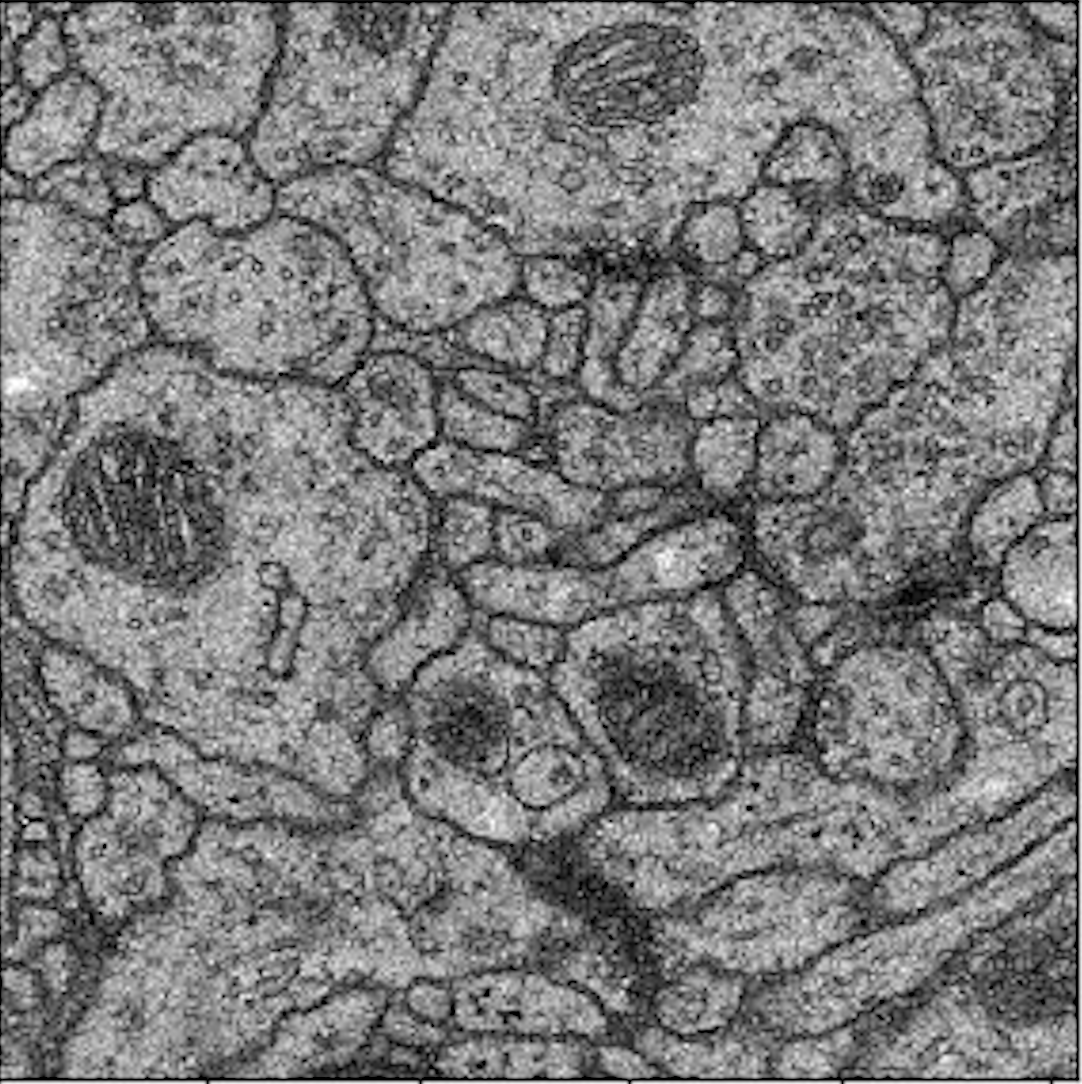
\includegraphics[width=.8\linewidth]{ISBIexampleRaw}
  \caption{Raw Image}
  \label{fig:ISBIexampleRaw}
\end{subfigure}%
\begin{subfigure}{.4\textwidth}
  \centering
  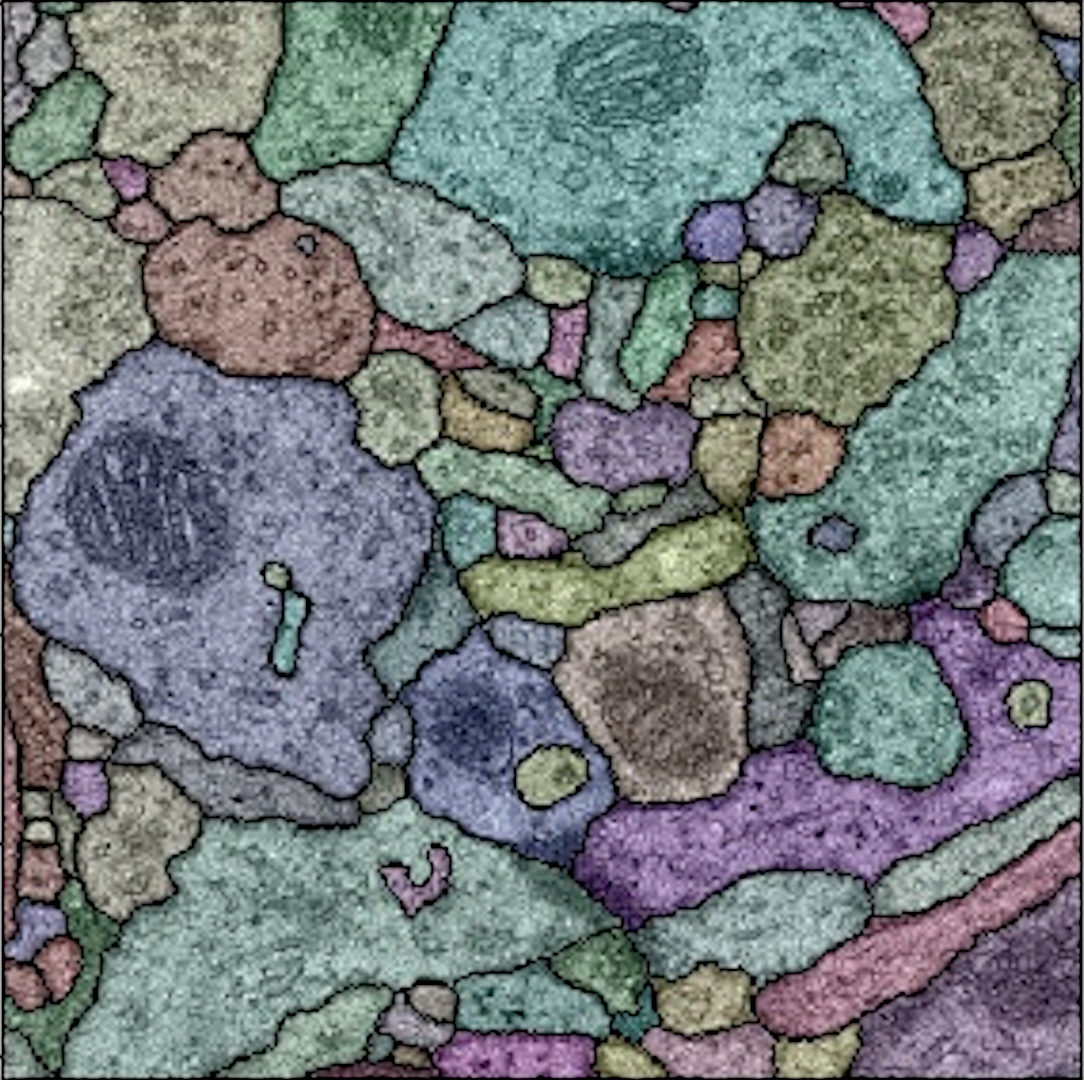
\includegraphics[width=.8\linewidth]{ISBIexampleGT}
  \caption{Ground Truth}
  \label{fig:ISBIexampleGT}
\end{subfigure}
\caption{An example of ISBI challenge Neuron Segmentation Problem}
\label{fig:ISBIexample}
\end{figure}


\paragraph{Hardware.} Fortunately I could lay my hand on a rusty, however relatively powerfull GTX970, and it did the work for me. However, I should add that as it can be seen in my code, my implementation is using a pretrained VGG network and this is for the following two reasons: First, in most of publications in Style Transfer, VGG network has sort of served as a benchmark so that the research community in this field could compare their result to each other. Second, training a network, requires a descent hardware, setting aside all the hyper parameter tuning that can appear in a practical implementation(which actually did appear for me because I first started with training my own implementation and realized this can't be done in the time frame of a mini project).

\paragraph{Structure.} The structure of this report is as follows: Section \ref{sec:theo} will have a short introduction to Deep Style Transfer and how does it generates the artistic style images along with some beautiful results from our beloved Heidelberg city, then I'll shortly introduce the Multicut method to solve Neuron Segmentation problem. Section \ref{sec:expe} will show the results of style transfer on the training set and Finally we'll have the result of inference on the augmented dataset  and compare that with the original dateset inference result.

\section{Theoretical Background}	
\label{sec:theo}

Machine Learning methods, and specifically Convolutional Neural Networks (CNNs) are showing promising results in a wide range of computer vision tasks, and are being used in different sectors. However, these methods works efficiently and with their best performance when they are fed with large-scale annotated data, a requirement that is not always easy to obtain. This is because preparing and labeling datasets are costly and there are ongoing challenges\cite{imageNet} which are meant to solve and automate this problem. On the other hand, there is also the data privacy which makes this task even more complicated, in which in sectors such Medical Image Analysis, normally patient data are secured by medical privacy laws which prevent any usage of the patients data in any open scientific tasks, and preparing dataset is pretty expensive and requires a collaboration of researchers and scientists\cite{DBLP}.

Data Augmentation methods are the solution for making synthetic data out of a small data set. There are different basic methods in augmenting data such as, flipping, rotating, scaling, translation, and so on; even adding random noise is considered as a form of data augmentation which usually result in reducing overfitting and improving the robustness of the system\cite{DBLP:journals/corr/abs-1712-03689}. In this project however, it's intended to augment the data set with \emph{styled} images of the data set.

\subsection{Artistic Style Transfer}

As it was mentioned earlier in the introduction section, there have recently been a lot of interest in the development of style transfer with the help of deep neural network. Based upon the innovative idea of Gatys et al, there have been two major stream lines of the developments, first being the development addressing the inefficiency of the computational process\citep{DBLP:journals/corr/UlyanovVL16}, and the capability of the algorithm to perform these artistic style transfers on videos. There were progress with utilizing the method of \emph{learning equivalent feed-forward generator networks} which can generate the stylized image in a single pass\citep{DBLP:journals/corr/JohnsonAL16, DBLP:journals/corr/UlyanovLVL16}. The second stream of the development was working on the so called \emph{photorealism} of the content image. This line of work concerns transferring the style of a reference photo to a content photo while maintaining faithfulness to the content image as much as possible\citep{Li}. For instance one can turn a photo of a city with skyscrapers full of windows in the daylight, to the exact same photo(faithfulness) but this time late in the night(figure \ref{fig:skyscrapers}). 

\begin{figure}[h]
	\centering
	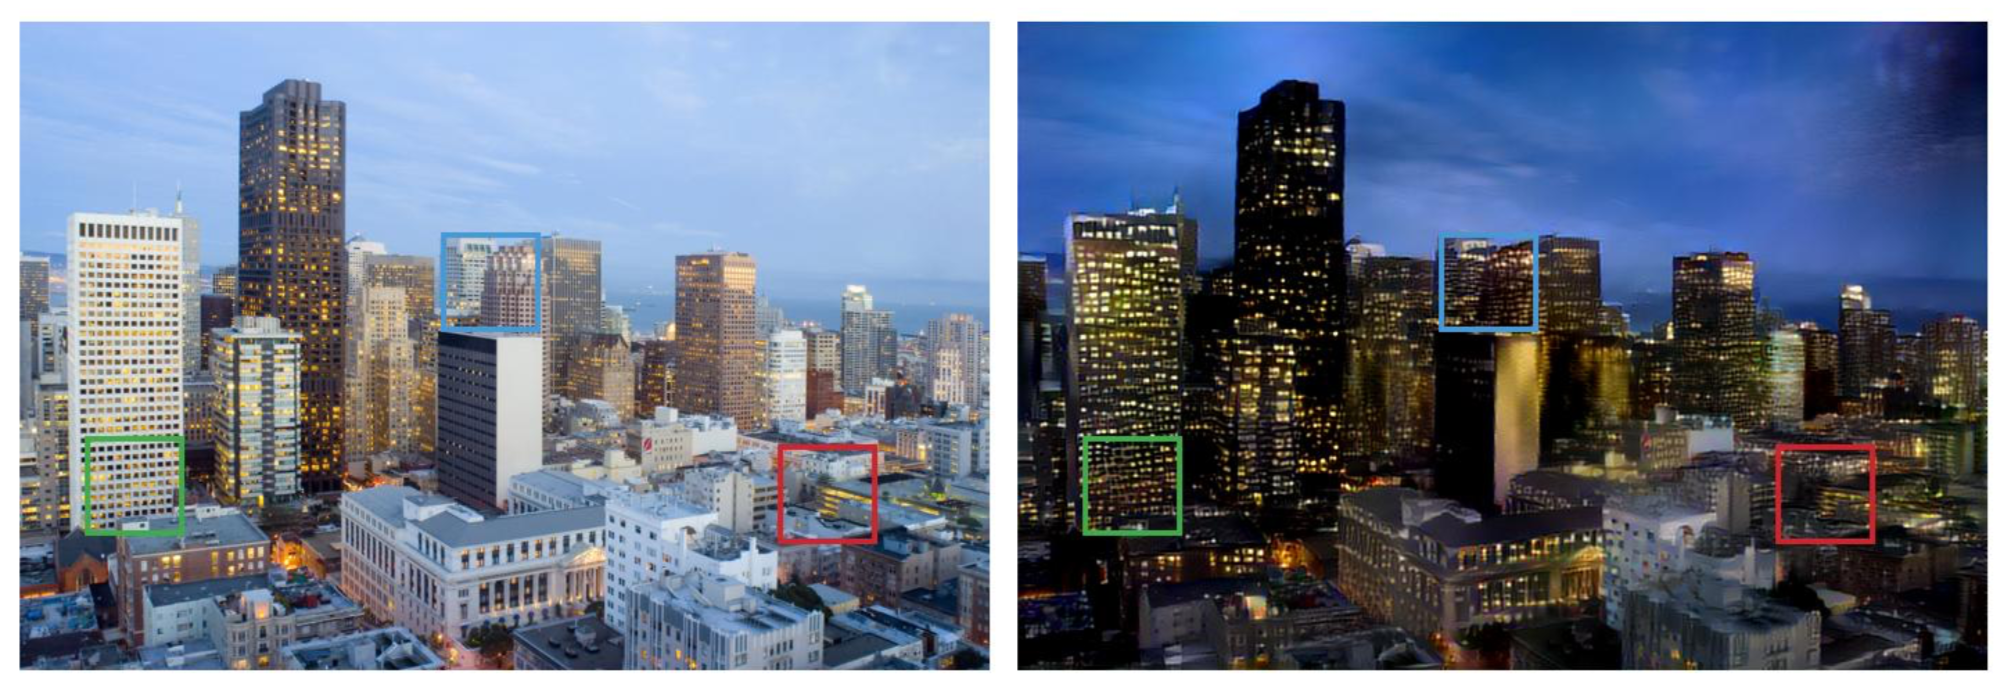
\includegraphics[width=0.7\textwidth]{skyscrapers}
	\caption{A photorealistic style transfer example. Image Credit \cite{Luan2017}}
	\label{fig:skyscrapers}
\end{figure}

In this work however, it is not intended to have a faithful style transfer, rather it's motivated to have unfaithful one, just like what Gatys et al. has published, paintings like with straight edges turns to wiggly and regular textures wavy\cite{Luan2017}. This is because I thought the more unfaithful the transfer is, the more ``informative'' the augmented data would be. This is why the implemented style transfer network is based on a Pytorch implementation of Gatys et al. work. 

The aim of their work was to generate a third image $x$ which has the content of image $p$ and the style of image $a$. This has been done by an energy minimization problem in which encoded the content loss and the style loss in it in the same time. The innovation in their work was to figure out that features extracted by a convolutional network carry information about the content of the image, while the correlations of these features encode the style\citep{Ruder}. Denoting $P^l$, $S^l$, and $F^l$ as the feature maps extracted by the network from the original image $p$, the style image $a$, and the stylized image $x$ we can formulate the content loss as equation \ref{equ:GatysLoss}, in which $N _ { l } \times M _ { l }$ denotes the dimensionality of these feature maps, $N _ { l }$ being the number of filters used, and  $M _ { l }$ being the spatial dimensionality of these feature maps, i.e the product of its width and height.

\begin{equation} \label{equ:GatysLoss}
\mathcal { L } _ { \text { content } } ( \boldsymbol { p } , \boldsymbol { x } ) = \sum _ { l \in L _ { \text { content } } } \frac { 1 } { N _ { l } M _ { l } } \sum _ { i , j } \left( F _ { i j } ^ { l } - P _ { i j } ^ { l } \right) ^ { 2 }
\end{equation}

This content loss, being the mean squared error between $P^l$ and $F^l$ doesn't need to be restricted to one layer, and as the equation \ref{equ:GatysLoss} shows, it's the sum of the mean squared error in all layers(set ${ L } _ { \text { content } } $) that is being used for content representation.

Coming to style loss, as we mentioned earlier, it's the mean squared error between \emph{correlation} of the filter responses, namely Gram matrices $A ^ { l } \in \mathbb { R } ^ { N _ { l } \times N _ { l } }$ for the style image $a$, and $G ^ { l } \in \mathbb { R } ^ { N _ { l } \times N _ { l } }$ for stylized image $x$ in which

\begin{equation} \label{equ:gramMatrices1}
	A _ { i j } ^ { l } = \sum _ { k = 1 } ^ { M _ { l } } S _ { i k } ^ { l } S _ { j k } ^ { l }
\end{equation}

\begin{equation} \label{equ:gramMatrices2}
	G _ { i j } ^ { l } = \sum _ { k = 1 } ^ { M _ { l } } F _ { i k } ^ { l } F _ { j k } ^ { l }
\end{equation}

and by having as in equation \ref{equ:GatysLoss} set ${ L } _ { \text { style } } $ as the set of layers used to represent the style, the style loss would be

\begin{equation} \label{equ:gatysStyleLoss}
\mathcal { L } _ {\text { style } } ( \boldsymbol { a } , \boldsymbol { x } ) = \sum _ { l \in L _ {\text { style } } } \frac { 1 } { N _ { l } ^ { 2 } M _ { l } ^ { 2 } } \sum _ { i , j } \left( G _ { i j } ^ { l } - A _ { i j } ^ { l } \right) ^ { 2 }
\end{equation}

and having them all together the loss function will be:

\begin{equation} \label{equ:gatysLoss}
\mathcal { L } _ { \text { singleimage } } ( \boldsymbol { p } , \boldsymbol { a } , \boldsymbol { x } ) = \alpha \mathcal { L } _ { \text { content } } ( \boldsymbol { p } , \boldsymbol { x } ) + \beta \mathcal { L } _ { \text {style} } ( \boldsymbol { a } , \boldsymbol { x } )
\end{equation}

in which $\alpha$ and $\beta$ are measures of importance for each component.

The image $x$ is generated by minimizing equation \ref{equ:gatysLoss} by a gradient-based optimization method. This is a straight forward description of Gatys method used in this project. The implementation can be found in the Github repository. Below you can see the output of this implementation with some beautiful photos of Heidelberg city, along with their style, and content itself.


%\begin{center}
%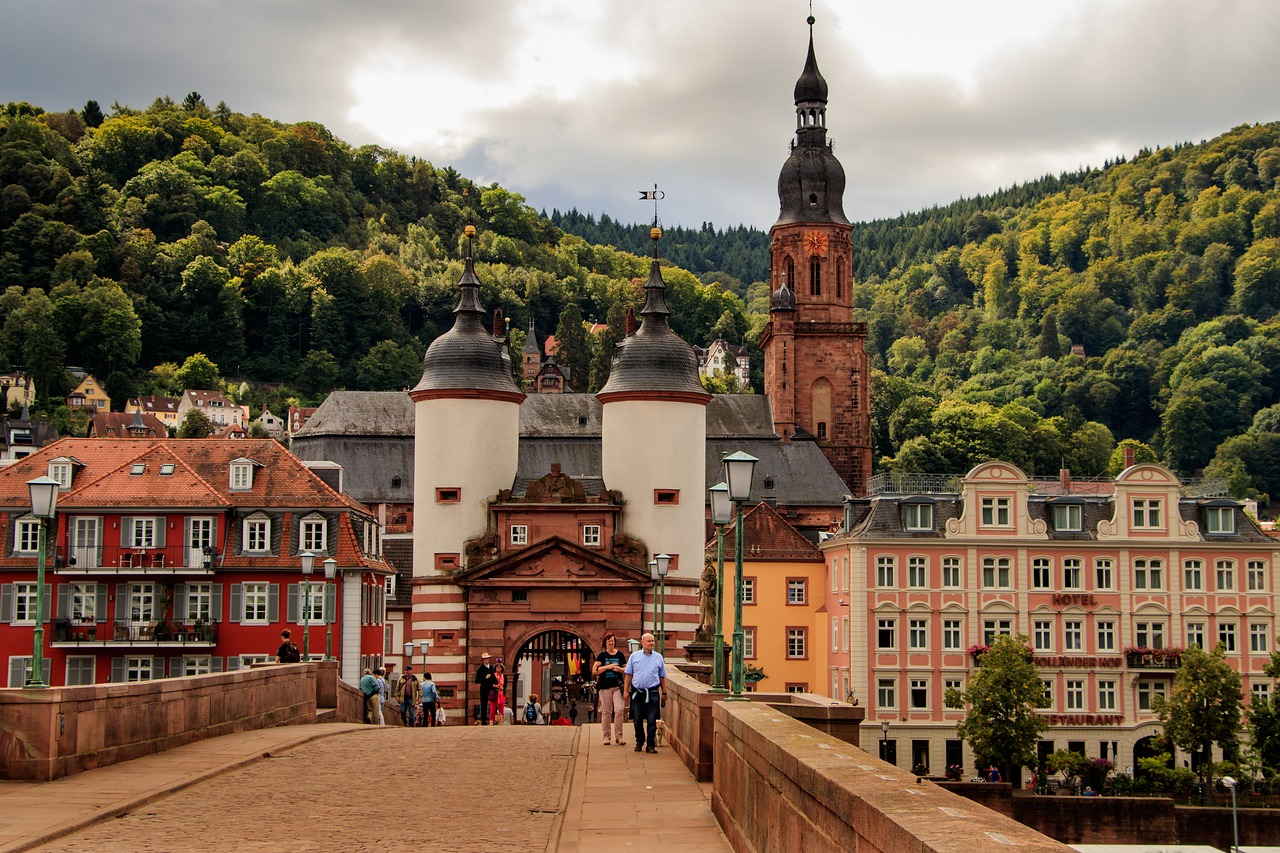
\includegraphics[width=5cm,height=5cm,keepaspectratio]{heidelberg2}\quad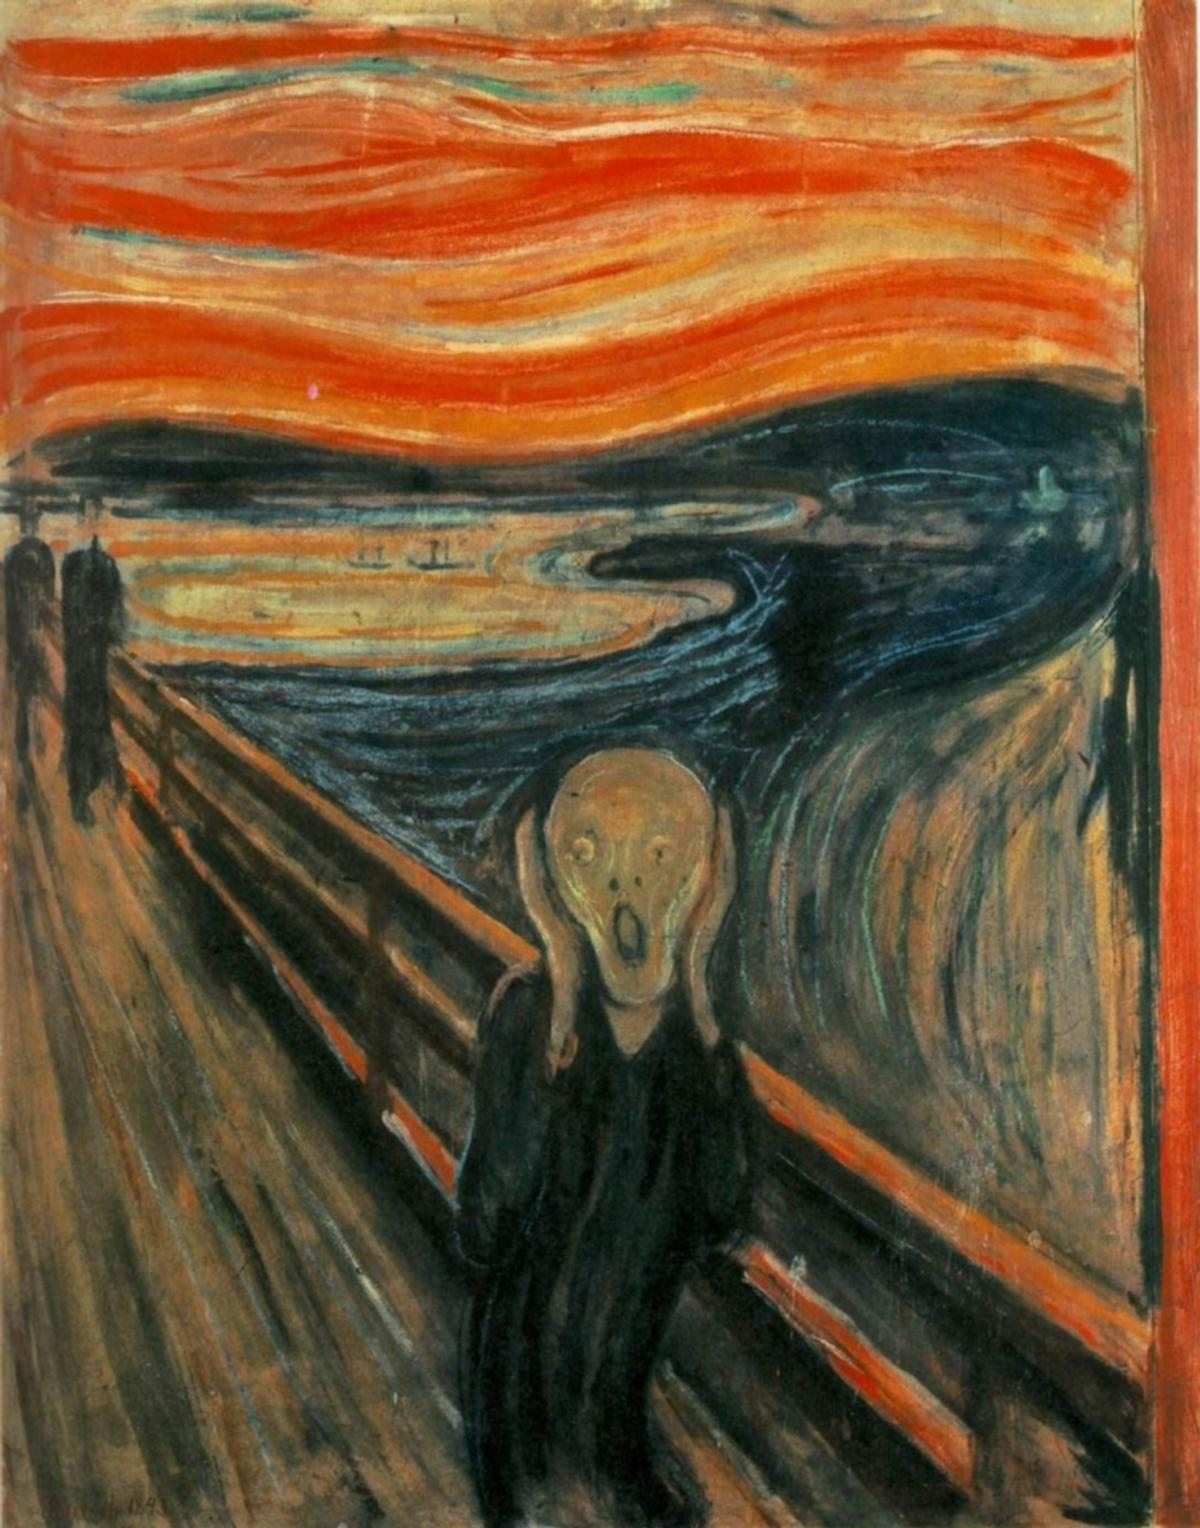
\includegraphics[width=3cm,height=3cm,keepaspectratio]{the_scream}\quad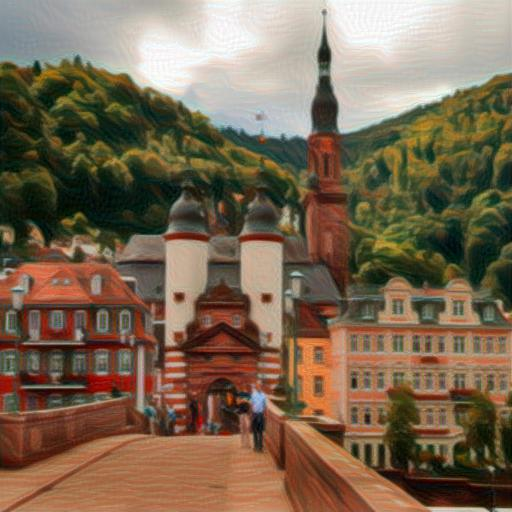
\includegraphics[width=5cm,height=5cm,keepaspectratio]{stylized-heidelberg2-the_scream}
%\\[\baselineskip]% adds vertical line spacing
%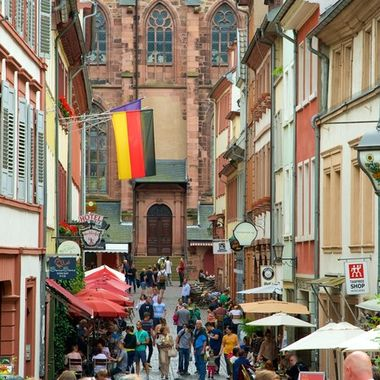
\includegraphics[width=5cm,height=5cm,keepaspectratio]{marktplatz}\quad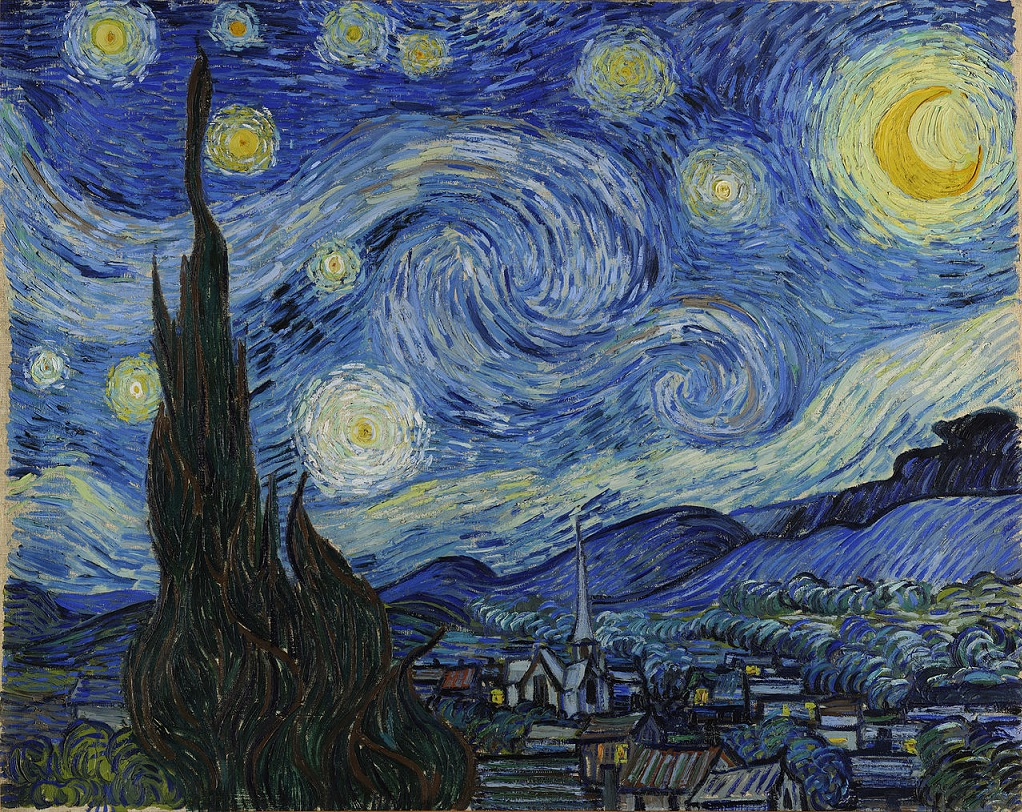
\includegraphics[width=3cm,height=3cm,keepaspectratio]{style2}\quad\includegraphics[width=5cm,height=5cm,keepaspectratio]{stylized-marktplatz-style2}
%\\[\baselineskip]% adds vertical line spacing
%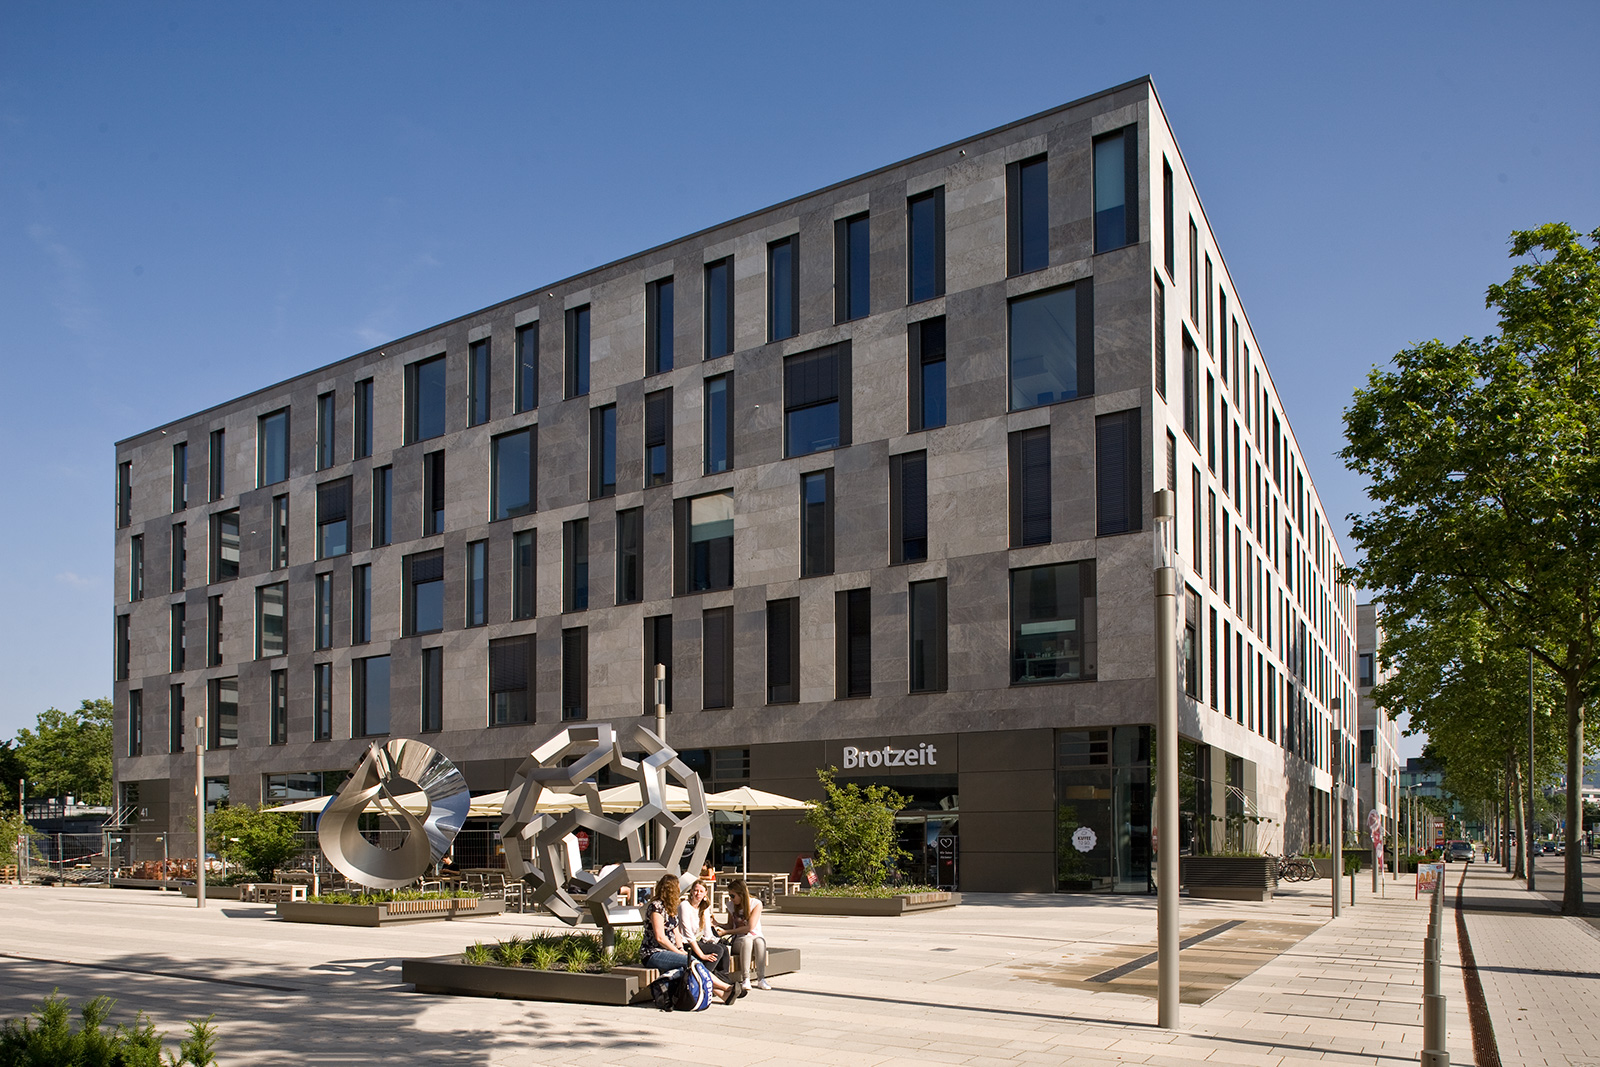
\includegraphics[width=5cm,height=5cm,keepaspectratio]{Mathematikon}\quad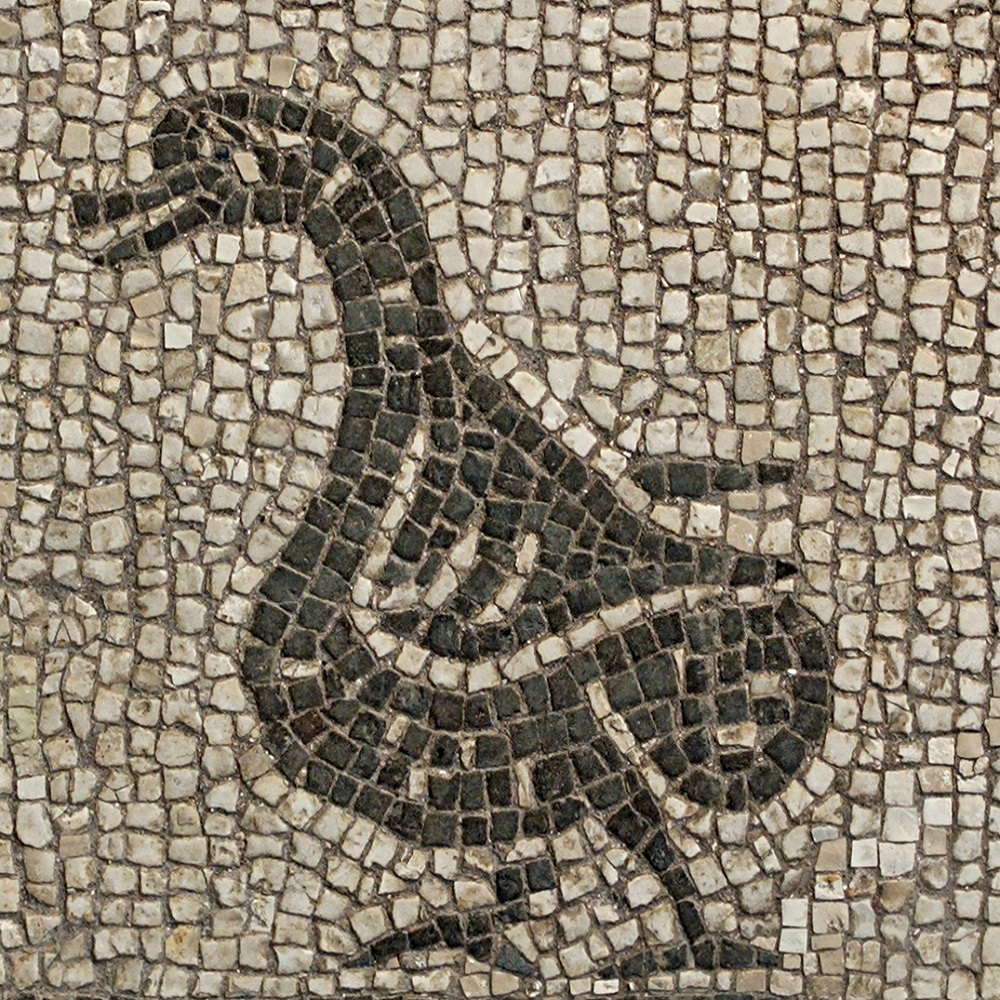
\includegraphics[width=3cm,height=3cm,keepaspectratio]{mosaic_ducks_massimo}\quad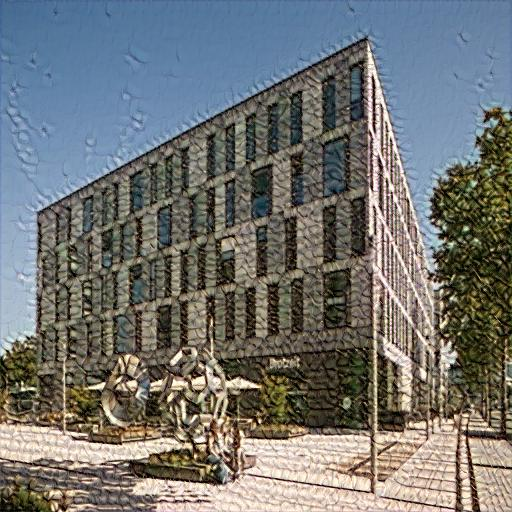
\includegraphics[width=5cm,height=5cm,keepaspectratio]{stylized-mathematikon-mosaic_ducks_massimo}
%%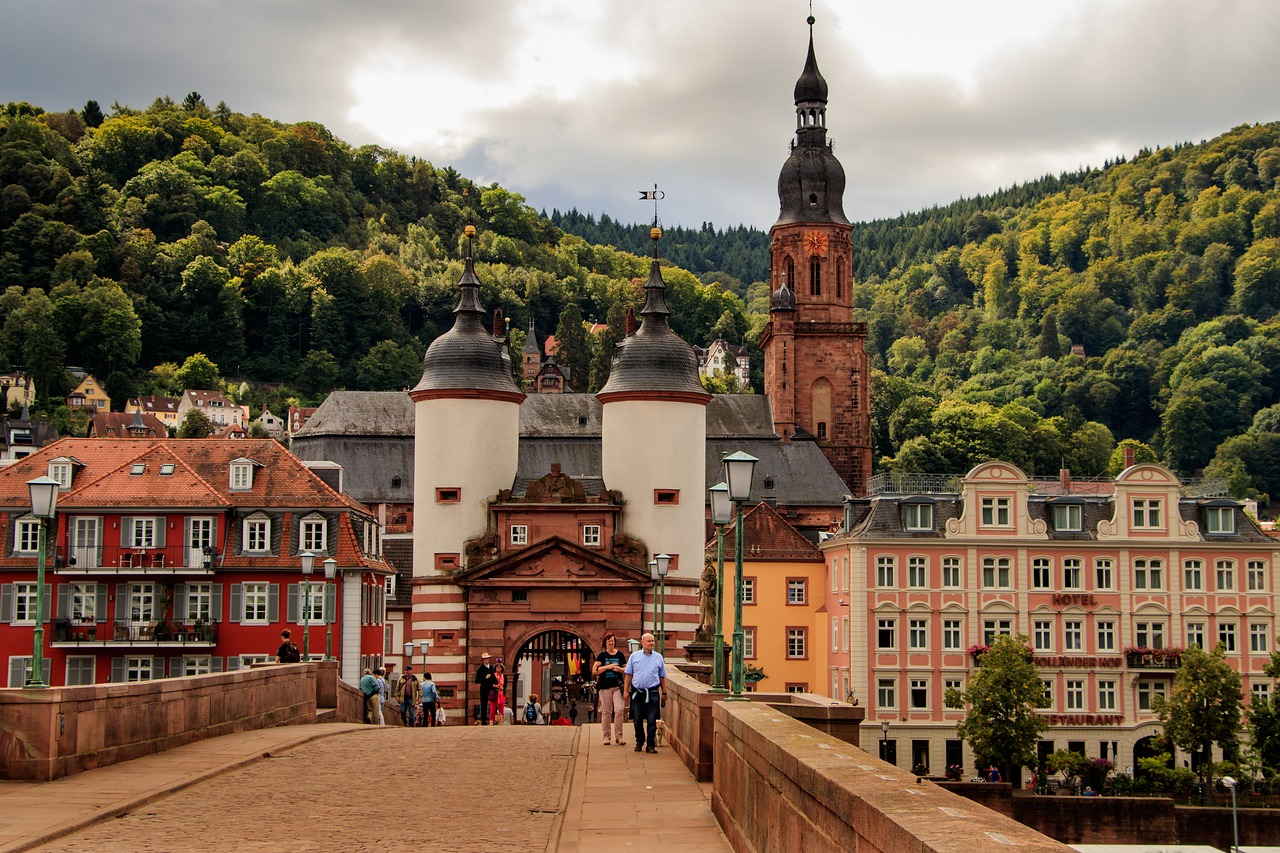
\includegraphics[width=.3\linewidth]{heidelberg2}\quad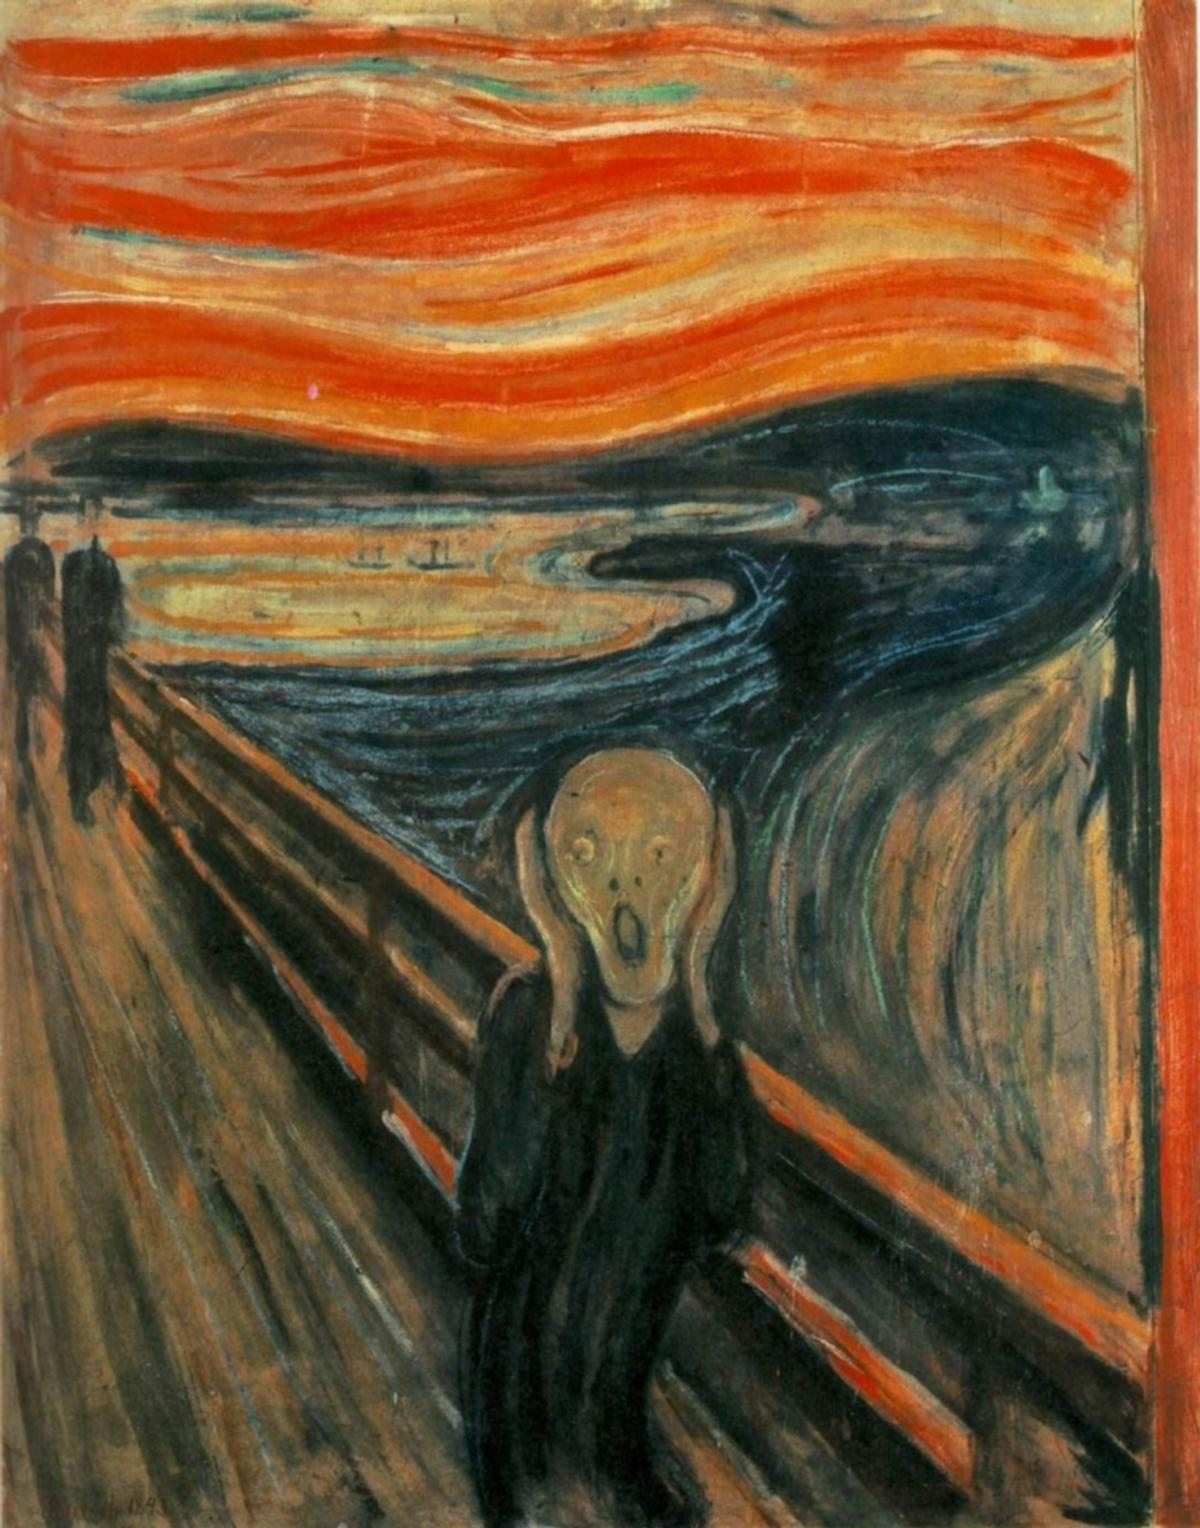
\includegraphics[width=.3\linewidth]{the_scream}\quad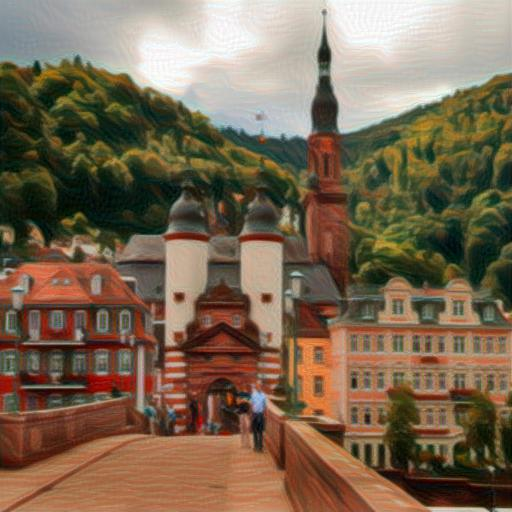
\includegraphics[width=.3\linewidth]{stylized-heidelberg2-the_scream}
%\end{center}

\begin{figure}[H]
\centering
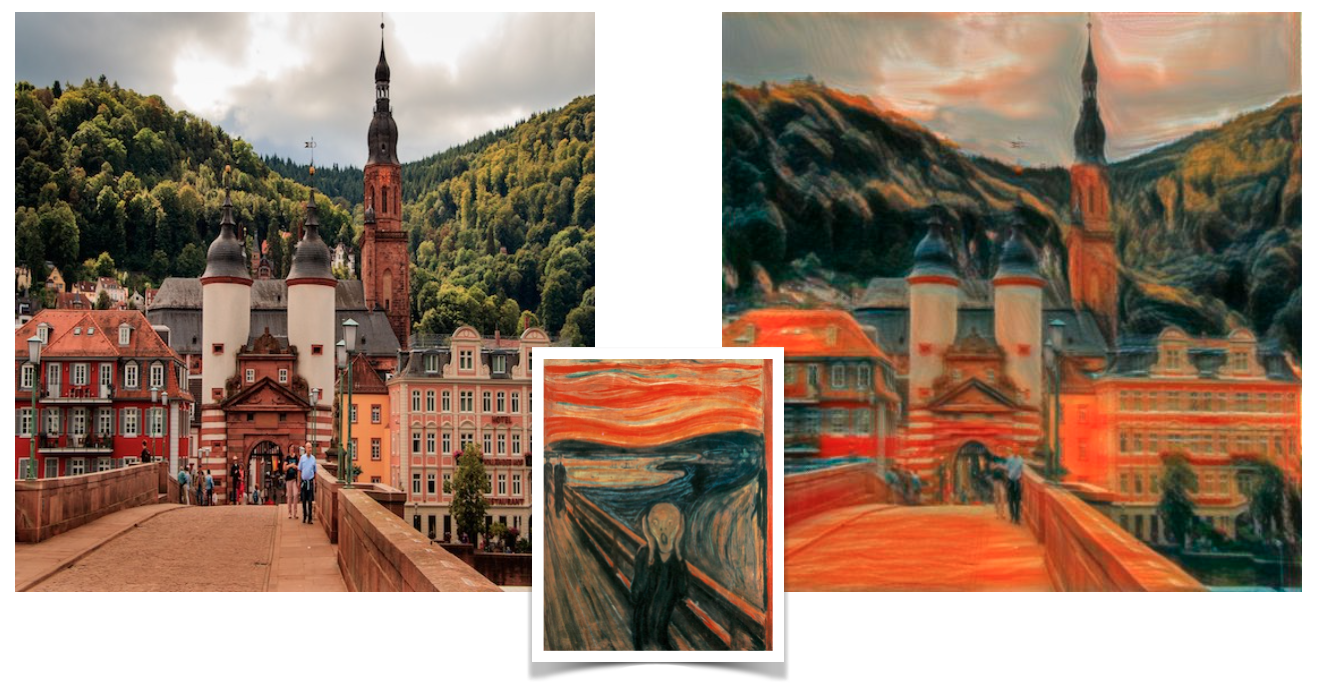
\includegraphics[width = .9\linewidth]{stylize1}
\caption{Stylized images using the VGG16 implementation\\ Left: Content Image, Center: Style Image, Right: Stylized Image}
\end{figure}


\begin{figure}[H]
\centering
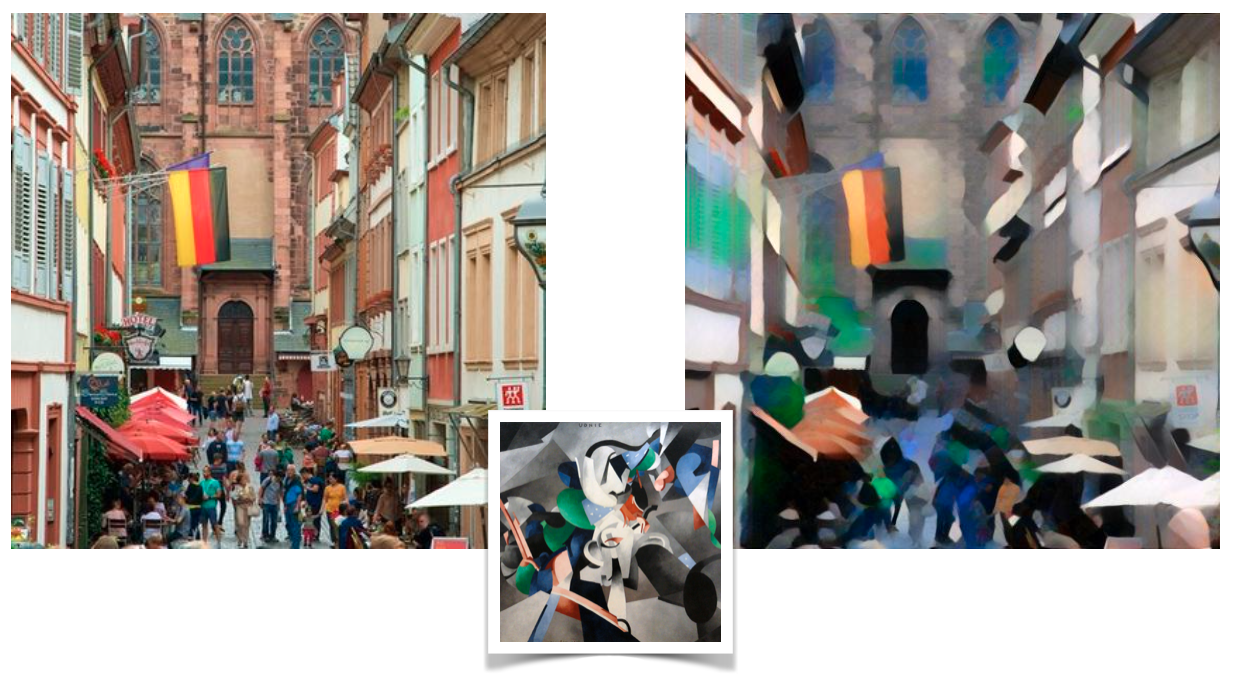
\includegraphics[width = .9\linewidth]{stylize2}
\caption{Stylized images using the VGG16 implementation\\ Left: Content Image, Center: Style Image, Right: Stylized Image}
\end{figure}

\begin{figure}[H]
\centering
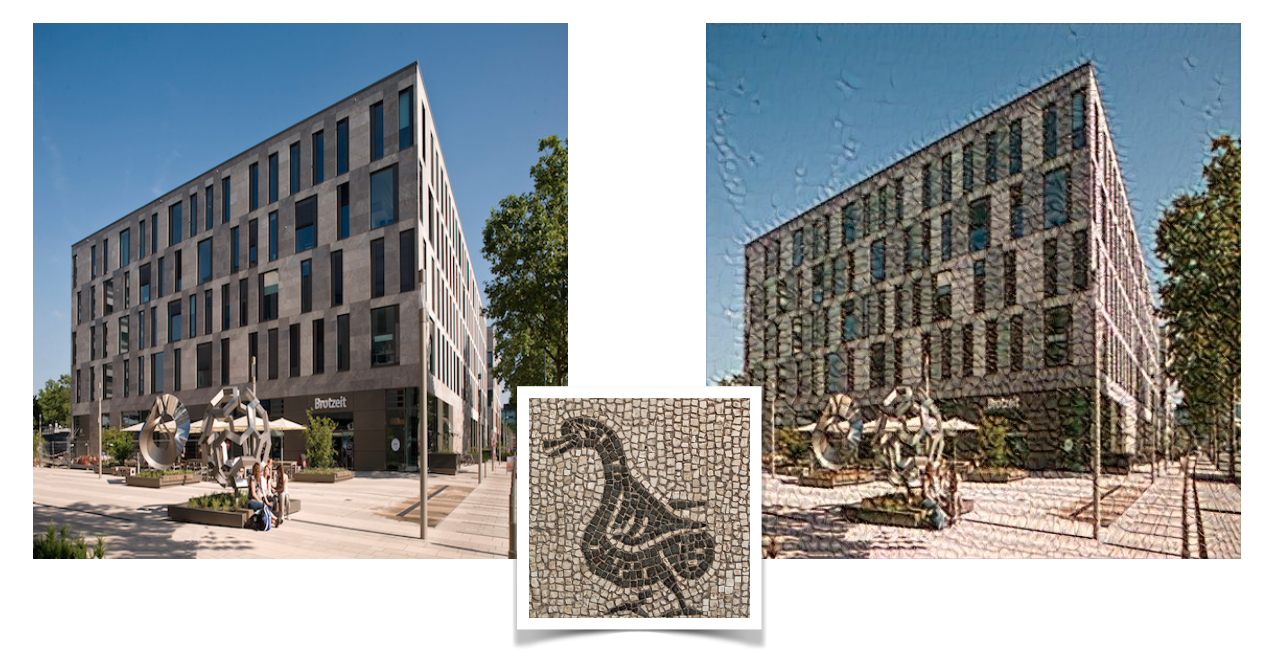
\includegraphics[width = .9\linewidth]{stylize3}
\caption{Stylized images using the VGG16 implementation\\ Left: Content Image, Center: Style Image, Right: Stylized Image}
\label{fig:stylizedImages_heidelberg}
\end{figure}


\subsection{Minimum Cost Multicut Problem}
\label{sec:multicut}
Beier et al. \citep{6078} has discussed the possibility of formulating an image segmentation problem as a minimum cost multicut problem on a designated graph. A short description of the method along with some definitions will be introduced here, for a detailed description refer to the original paper or to \citep{26, 27}. Applying a basic segmentation technique (e.g. watershed segmentation) on an image will result in a segmented image in which each segmentation contains a group of pixels with a very similar neighbouring characteristics. However as it is usually the case, applying these methods on our raw image of the training set(figure \ref{fig:ISBIexampleRaw}) will result in the so called over segmentation, which means the actual segmentation that we are looking for will be segmented in many other small segmentation. In a minimum cost multicut problem, we try to assign each of these super pixels to a \emph{node} in our graph, and connect each of these nodes to the neighbouring nodes(super pixels) with an \emph{edge}. This way we will wind up with a graph designated to the raw image and we'll try to apply our learning problem on this graphs in a sense that a probability of how probable each edge to be ``true'' is calculated and learned, and whenever this probabilty is lower than a specific threshhold, the edge will be ``cut'' and the two super pixels would merge in one bigger super pixel. \\

The final/optimal solution to the problem is the solution to the optimization problem whose feasible solution is the proper decomposition of the graph. In a mathematical formulation, defining each graph as $G = (V, E)$ in which $V$ denotes the set of nodes, $E$ denotes the set of edges, and every $c : E \rightarrow \mathbb { R }$, the optimization problem designated for the minimum cost multicut problem would be

\begin{equation} \label{equ:multicutProblem}
\begin{array} { c l } { \min _ { x \in \{ 0,1 \} ^ { E } } } & { \sum _ { e \in E } c _ { e } x _ { e } } \\  \\{ \text { subject to } } & { \forall Y \in \operatorname { cycles } ( G ) \forall e \in Y : x _ { e } \leq \sum _ { e ^ { \prime } \in Y \backslash \{ e \} } x _ { e ^ { \prime } } } \end{array}
\end{equation}

\section{Experiments \& Discussion}
\label{sec:expe}

As it is discussed in section \ref{sec:multicut}, first step to convert an image to a graph is to apply some sort of basic segmentation method. In order to do that, the implementation uses the NIFTY software \citep{niftyDoc} in which it first uses the watershed segmentation method and turns the raw image to an over-segmented image:
\begin{figure}[H]
\centering
\begin{subfigure}{.45\textwidth}
  \centering
  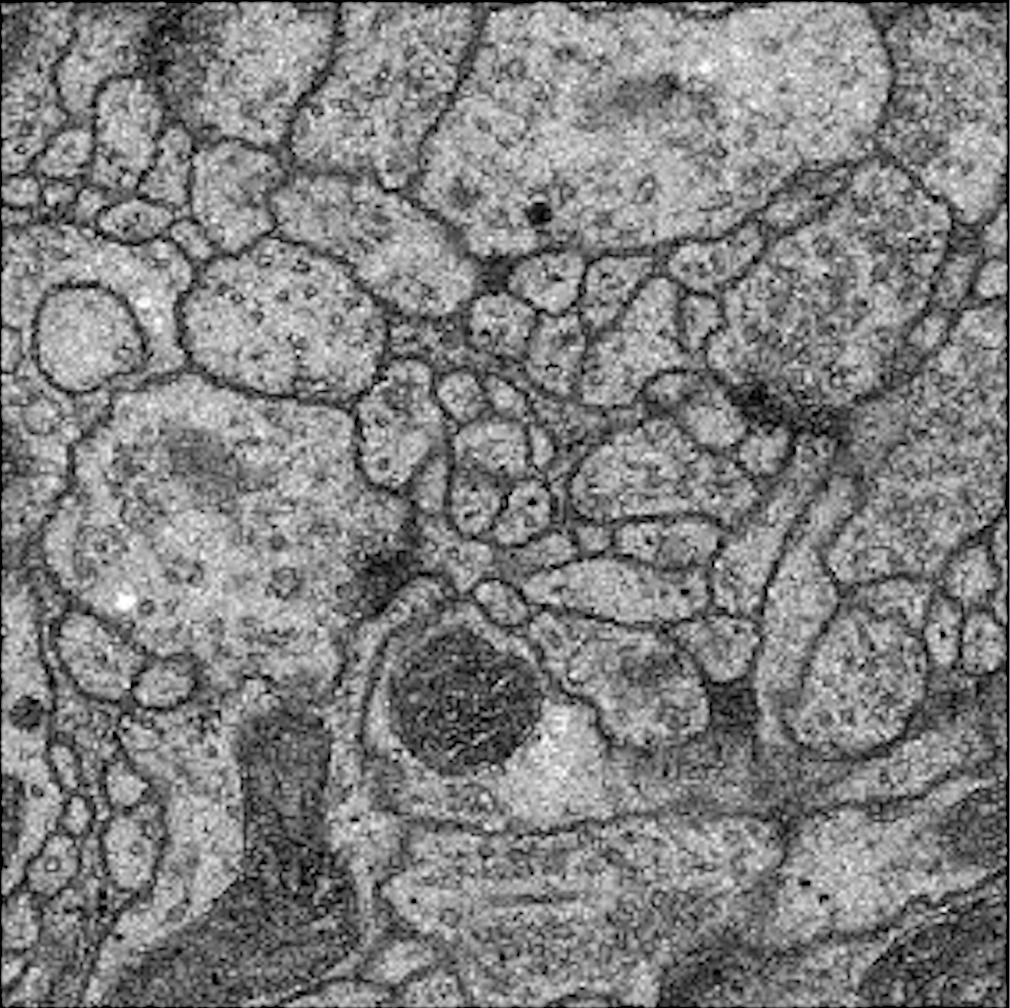
\includegraphics[width=.8\linewidth]{os1}
  \caption{Raw Image}
  \label{fig:os1}
\end{subfigure}%
\begin{subfigure}{.45\textwidth}
  \centering
  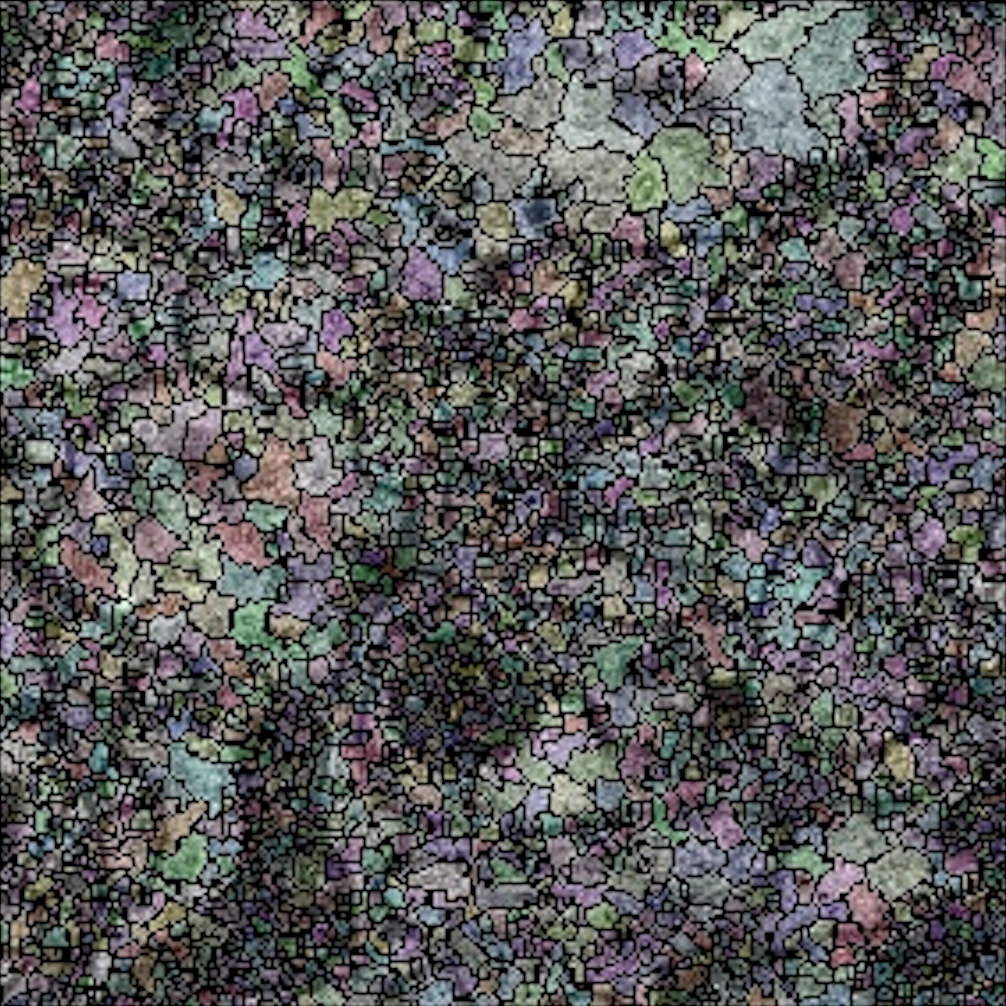
\includegraphics[width=.8\linewidth]{os2}
  \caption{Oversegmented Image}
  \label{fig:os2}
\end{subfigure}

\label{fig:oversegment}
\caption{Watershed Segmentation Result}
\end{figure}


However, this results in a really big graph with thousands of edges, and applying this to our whole data set would result in a really huge training set of millions of instances. In order to avoid that, a \emph{Frangi} filter \citep{scikit} has been applied on the images in advance, so that it results in a bigger segmented super pixels.

\begin{figure}[H]
\centering
\begin{subfigure}{.3\textwidth}
  \centering
  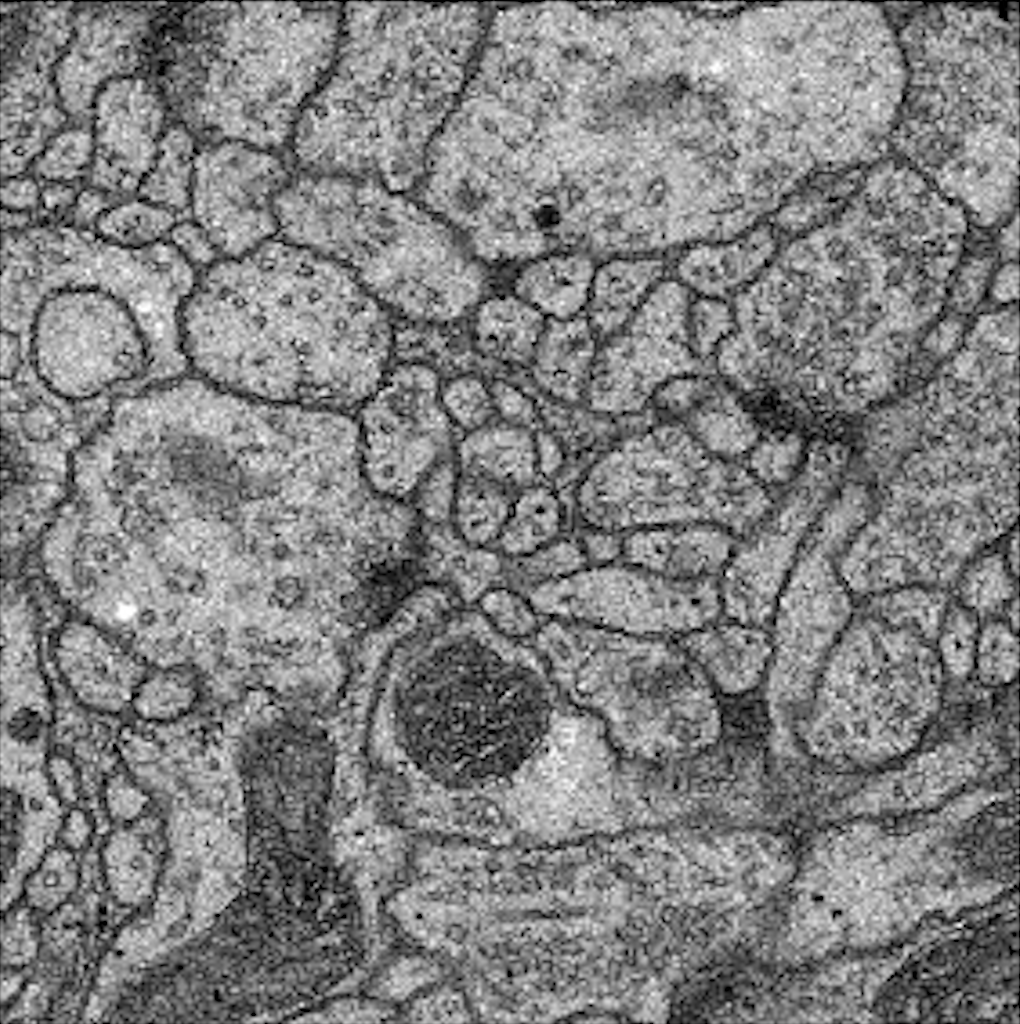
\includegraphics[width=.9\linewidth]{frangi1}
  \caption{Raw Image}
  \label{fig:frangi1}
\end{subfigure}%
\begin{subfigure}{.3\textwidth}
  \centering
  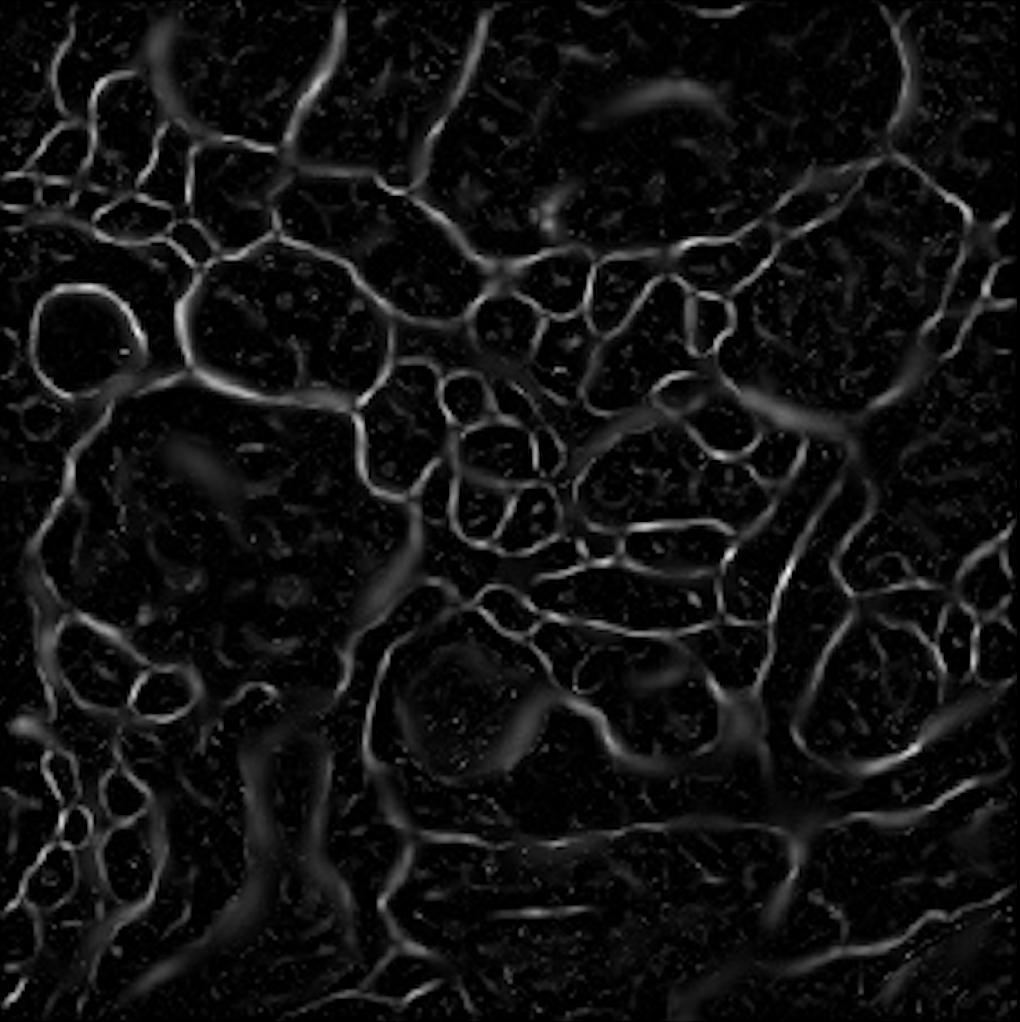
\includegraphics[width=.9\linewidth]{frangi2}
  \caption{Frangi Filtered Image}
  \label{fig:frangi2}
\end{subfigure}
\begin{subfigure}{.3\textwidth}
  \centering
  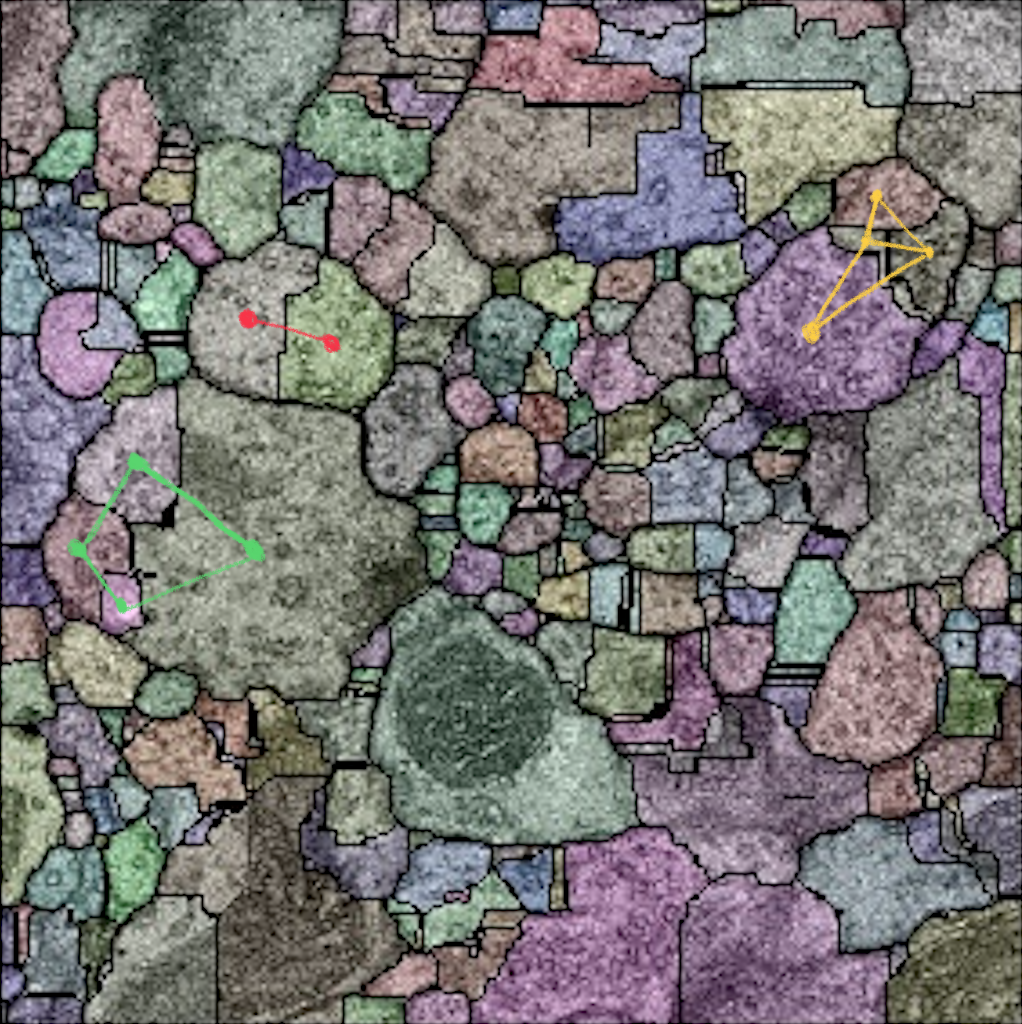
\includegraphics[width=.9\linewidth]{frangi3}
  \caption{Oversegmented Image}
  \label{fig:frangi3}
\end{subfigure}

\label{fig:frangi}
\caption{Watershed segmentation result with Frangi filter applied}
\end{figure}

Keeping in mind figure \ref{fig:ISBIexampleGT} for the ground truth image, the objective is learning to \emph{cut} the edges in the over-segmented image(figure \ref{fig:frangi3}) which does not have a high probability of being an edge. Some of this edges have been drawn on figure \ref{fig:frangi3} with blue, green and yellow hand sketches.

\subsection{Style Transfer on Raw Images}

Right out of the bat, after I've seen the results of style transfer on the neuron images, I sort of realized this wouldn't introduce \emph{informative} data to the training set. Reason being is the neuron edges did not move that much that I was expecting, therefore the whole style transfer acted as a filter to the image. For this reason, I tried to apply many different style images on the raw data, with different optimization step numbers, hoping that I could end up with more informative images, however with no avail. Below you can see some of the results of these style transfers:

\begin{figure}[H]
\centering
\begin{subfigure}{.34\textwidth}
  \centering
  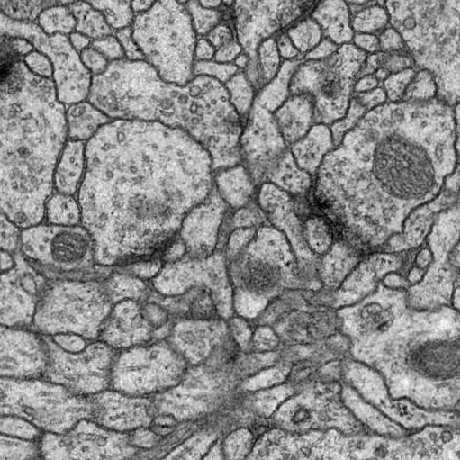
\includegraphics[width=.9\linewidth]{ISBI0}

  \label{fig:nas31}
\end{subfigure}%
\begin{subfigure}{.28\textwidth}
  \centering
  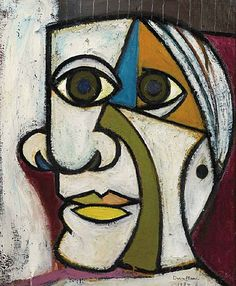
\includegraphics[width=.9\linewidth]{style3}

  \label{fig:nas32}
\end{subfigure}
\begin{subfigure}{.34\textwidth}
  \centering
  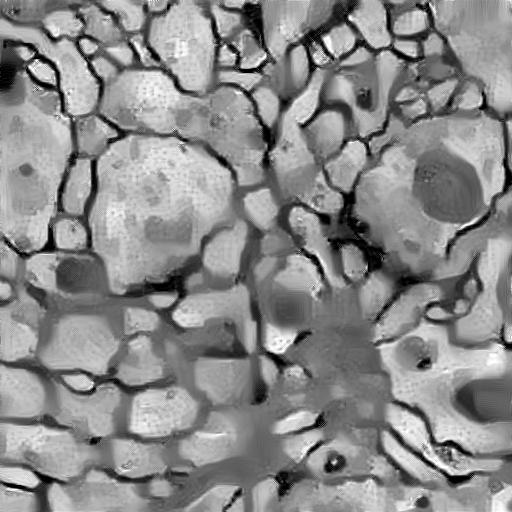
\includegraphics[width=.9\linewidth]{stylized-train0-style3-150}

  \label{fig:nas33}
\end{subfigure}
\label{fig:neuron_art_style3}
\end{figure}

\begin{figure}[H]
\centering
\begin{subfigure}{.34\textwidth}
  \centering
  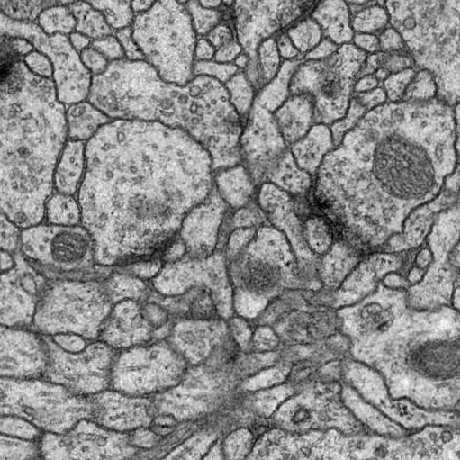
\includegraphics[width=.9\linewidth]{ISBI0}

  \label{fig:nas101}
\end{subfigure}%
\begin{subfigure}{.28\textwidth}
  \centering
  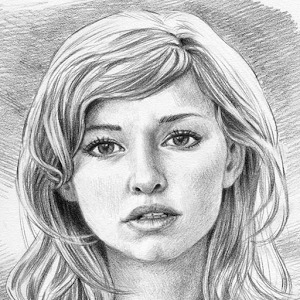
\includegraphics[width=.99\linewidth]{style10}

  \label{fig:nas102}
\end{subfigure}
\begin{subfigure}{.34\textwidth}
  \centering
  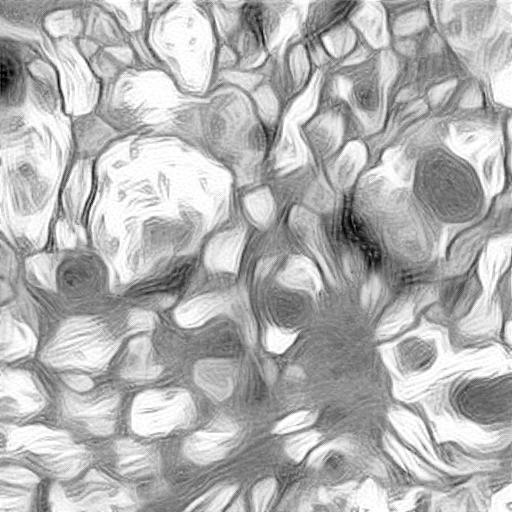
\includegraphics[width=.9\linewidth]{stylized-train0-style10-150}

  \label{fig:nas103}
\end{subfigure}
\label{fig:neuron_art_style10}
\end{figure}

\begin{figure}[H]
\centering
\begin{subfigure}{.34\textwidth}
  \centering
  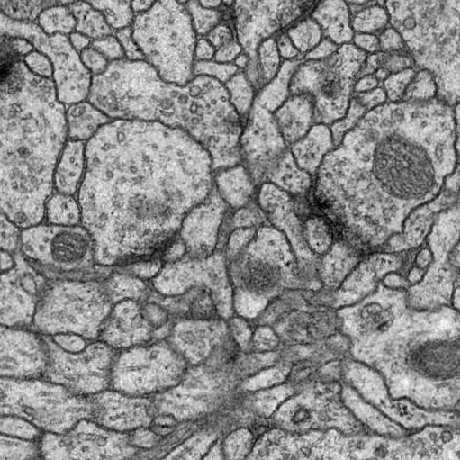
\includegraphics[width=.9\linewidth]{ISBI0}
  \caption{Raw Image}
  \label{fig:nas211}
\end{subfigure}%
\begin{subfigure}{.28\textwidth}
  \centering
  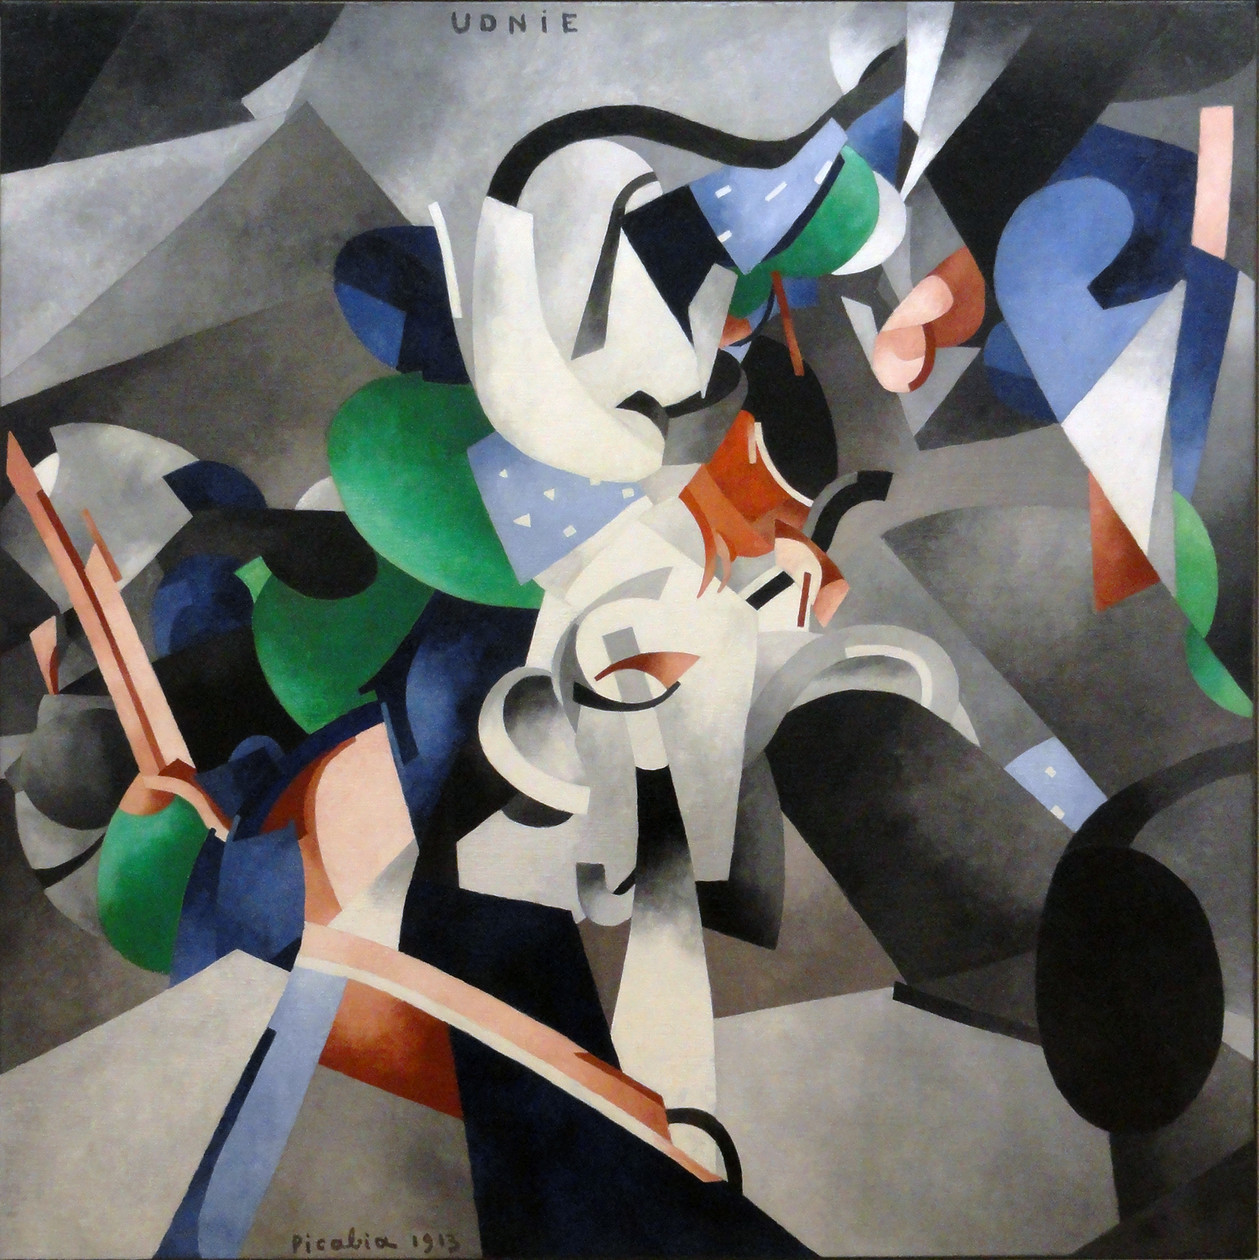
\includegraphics[width=.99\linewidth]{udnie}
  \caption{Style Image}
  \label{fig:nas212}
\end{subfigure}
\begin{subfigure}{.34\textwidth}
  \centering
  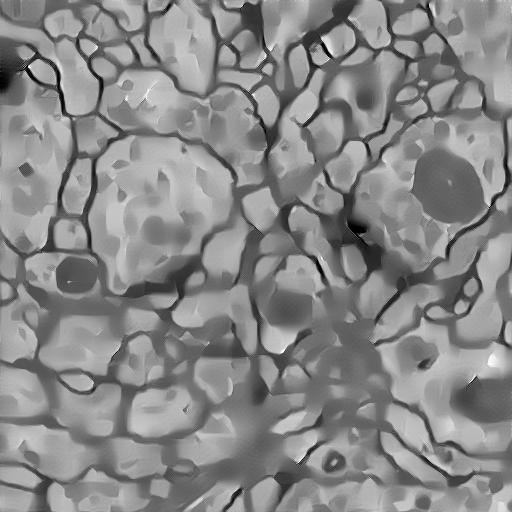
\includegraphics[width=.9\linewidth]{stylized-train0-style21-150}
  \caption{Stylized Image}
  \label{fig:nas213}
\end{subfigure}
\label{fig:neuron_art_style21}
\caption{Artistic Style Transfer on neuron images}
\end{figure}

The whole dataset has went through style transfer on 24 style images \citep{21styles} with two different optimization number of steps (75, 150) and can be seen in the project Github repository. The smoothness achieved by transferring the style of artistic paintings to the raw images made me think that transferring images with continuous textures would act as a sort of filter to the image, this way we might use these styled transferred images with out applying Frangi filter on them. However the result wasn't satisfying either and can be seen for different styles \citep{textureStyles} on the Github repository. 

\subsection{Result of Data Augmentation}

In this section, various scenarios has been tested in an attempt to seek better results than the original inference. However, first we'll see how the result of the segmentation before augmenting the dataset is. As being mentioned earlier, the result with oversegmented(without applying Frangi filter) is not satisfying, 


\begin{figure}[H]
\centering
\begin{subfigure}{.35\textwidth}
  \centering
  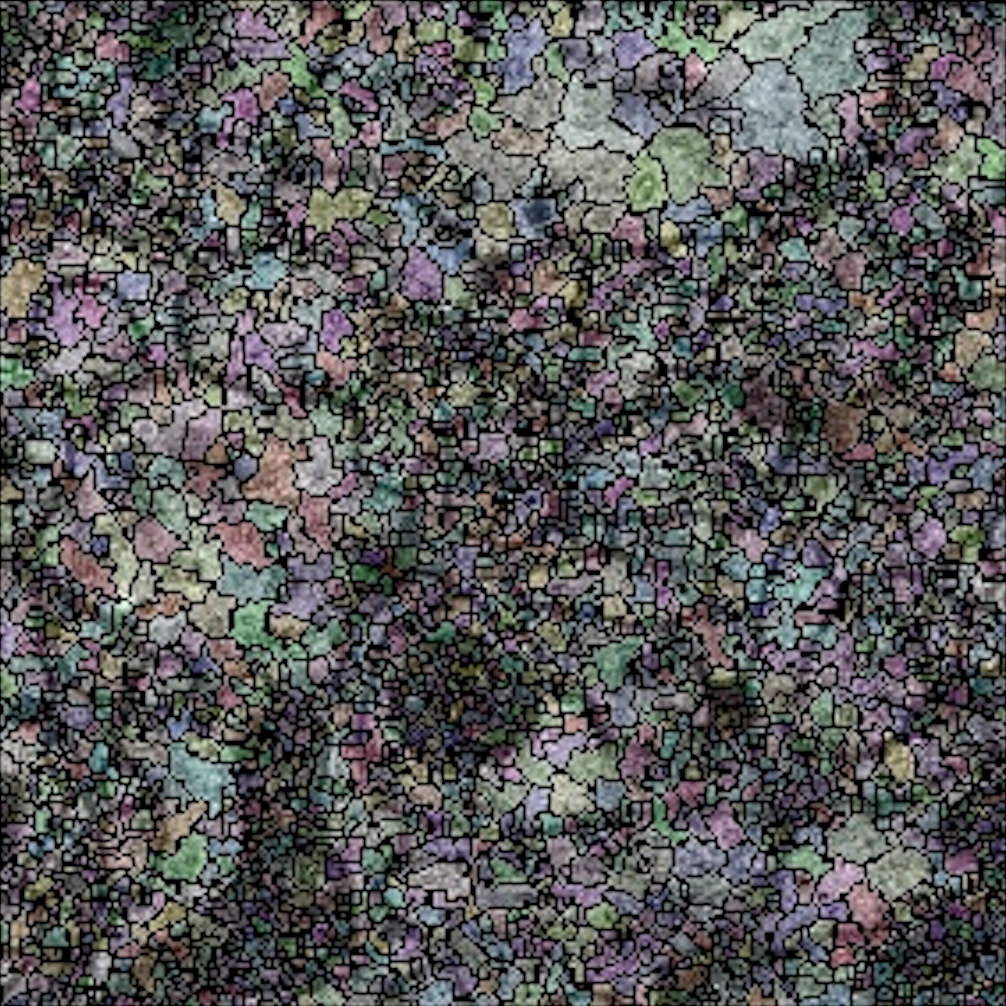
\includegraphics[width=.8\linewidth]{os2}
  \label{fig:os1}
\end{subfigure}%
\begin{subfigure}{.35\textwidth}
  \centering
  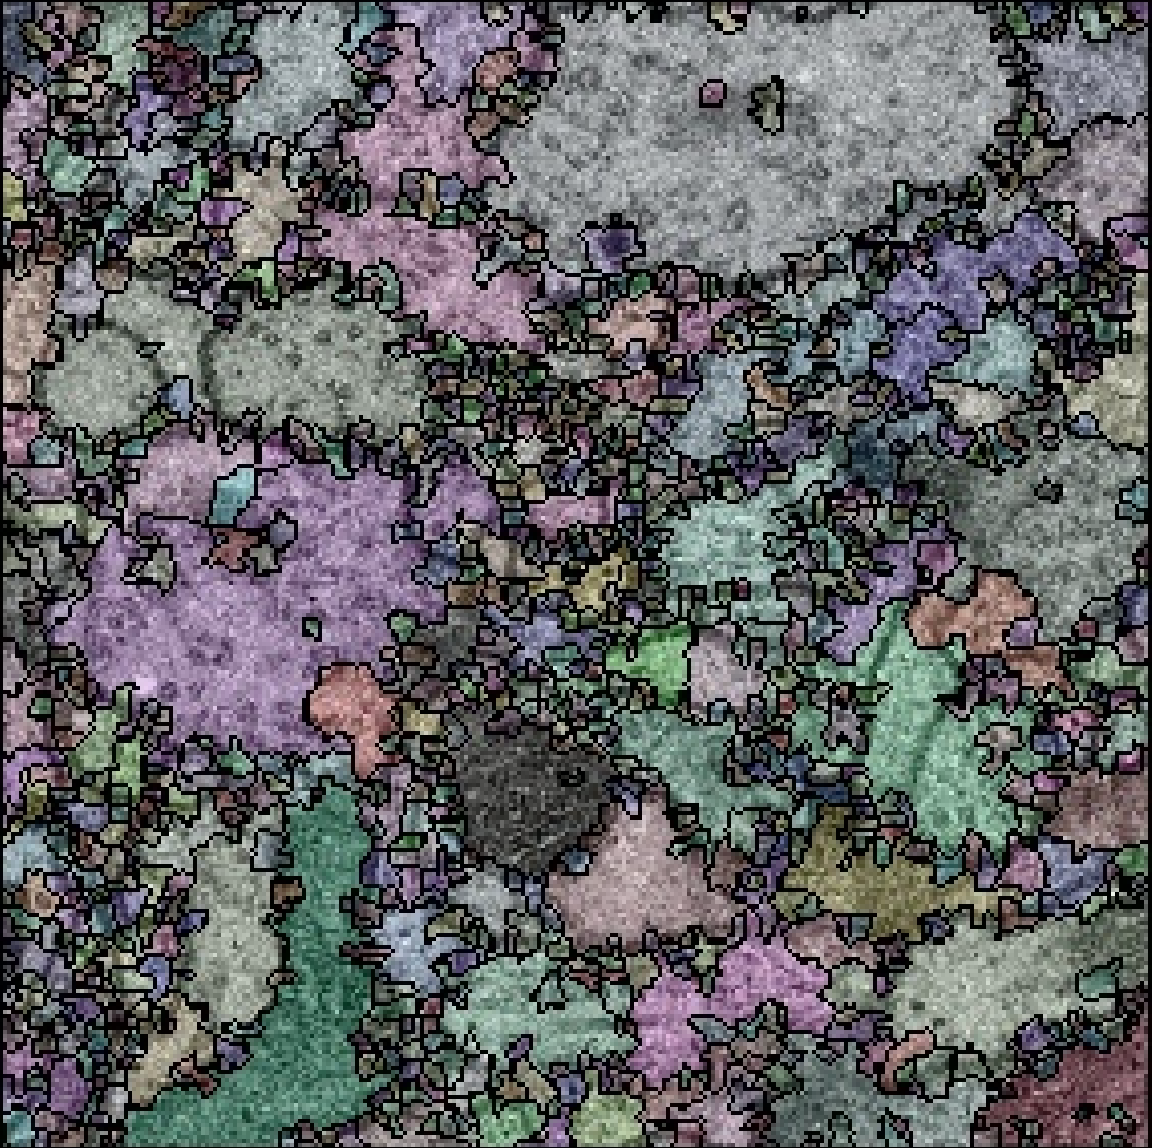
\includegraphics[width=.8\linewidth]{os3}
  \label{fig:os2}
\end{subfigure}

\label{fig:oversegment}
\caption{Inference on oversegmented(without Frangi) image}
\end{figure}

and we applied Frangi filter to obtain the oversegmented image and applying the inference with 24 images as training set we will obtain:

\begin{figure}[H]
\centering
\begin{subfigure}{.3\textwidth}
  \centering
  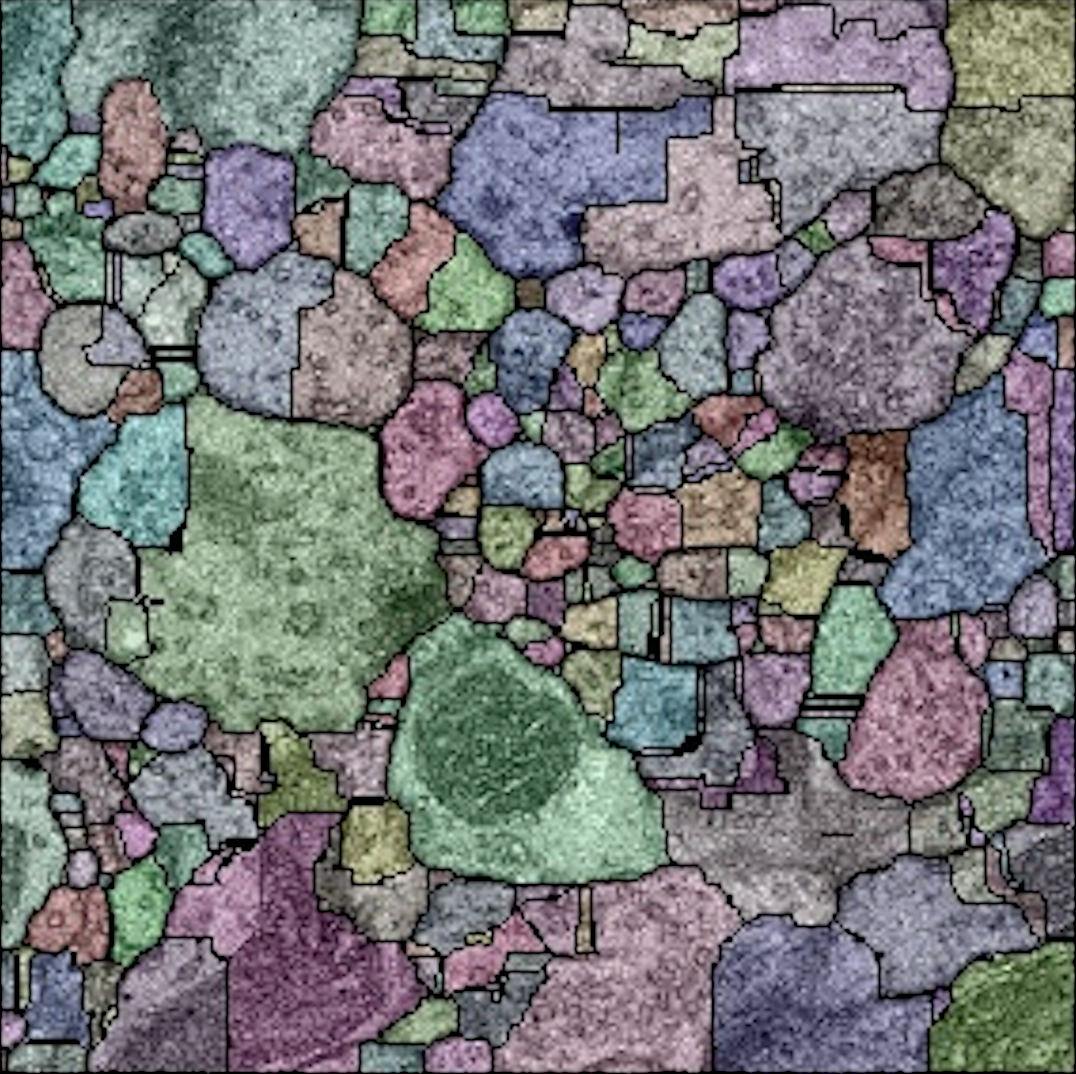
\includegraphics[width=.9\linewidth]{oi1}
  \caption{Oversegmented Image}
  \label{fig:oi1}
\end{subfigure}%
\begin{subfigure}{.3\textwidth}
  \centering
  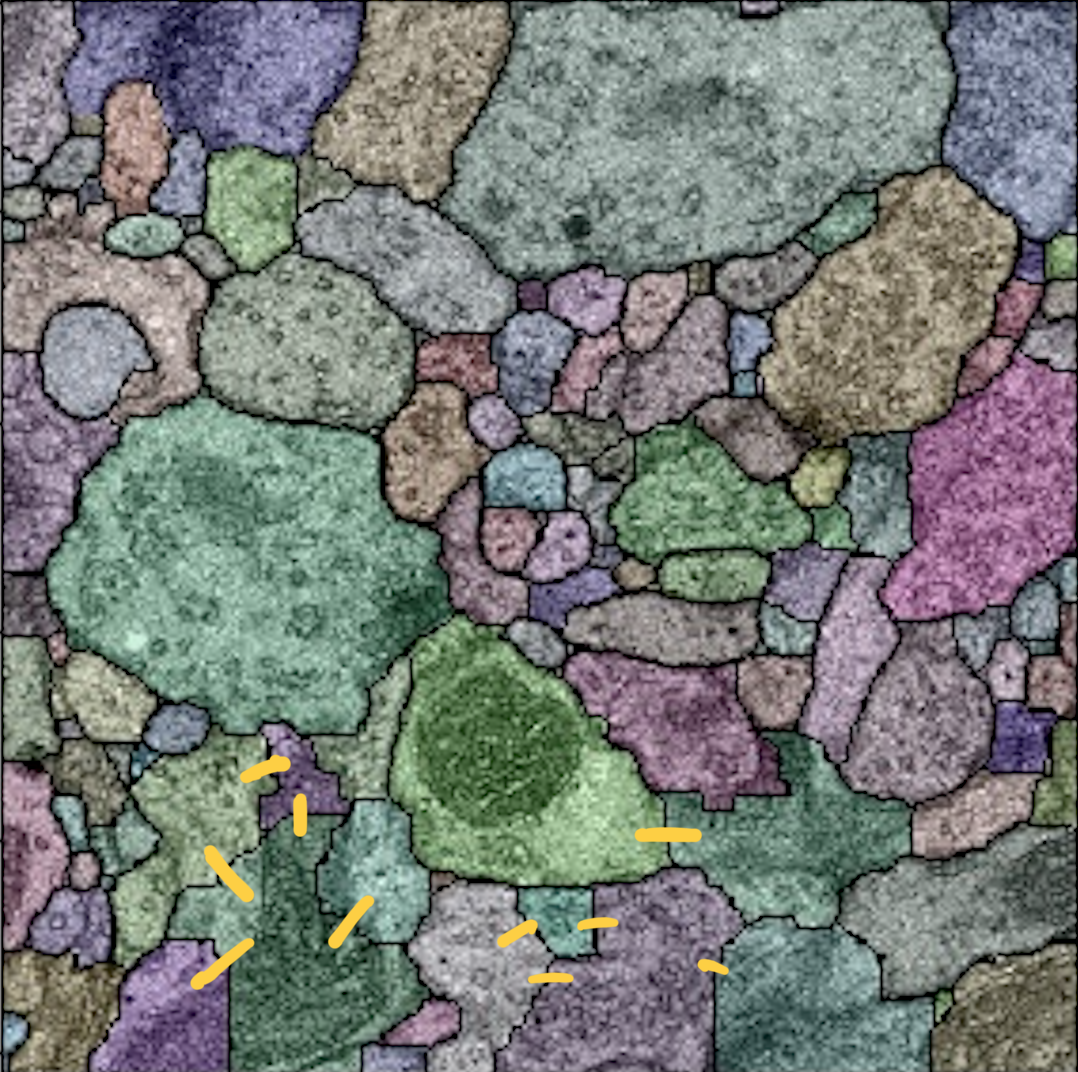
\includegraphics[width=.9\linewidth]{oi22}
  \caption{Inference Image}
  \label{fig:oi2}
\end{subfigure}
\begin{subfigure}{.3\textwidth}
  \centering
  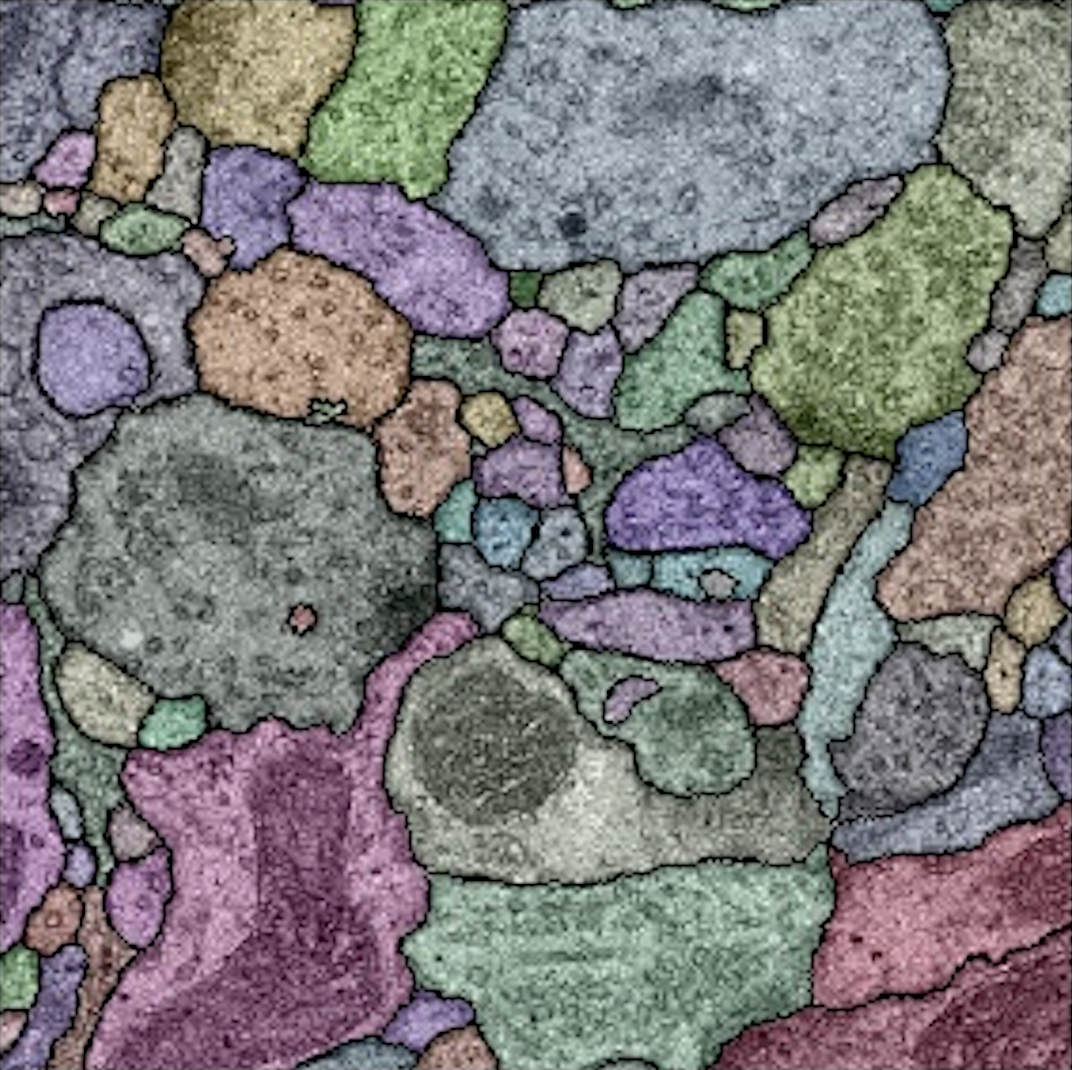
\includegraphics[width=.9\linewidth]{oi3}
  \caption{Ground Truth Image}
  \label{fig:oi3}
\end{subfigure}

\label{fig:original_inference}
\caption{Inference result with the original dataset}
\end{figure}

As it is shown in figure \ref{fig:oi2}, the inference is doing a pretty good job in general, however there are some edges(e.g. edges marked in yellow on figure \ref{fig:oi2}) that needs to be cut and I was hoping I could improve the inference with the data augmentation.

My first attempt was of course augmenting all the stylized images to the main data set, this way we obtain 600 images from 24 images (including the original image itself). Below you can see the result of this inference comparing to the original inference.

\begin{figure}[H]
\centering
\begin{subfigure}{.3\textwidth}
  \centering
  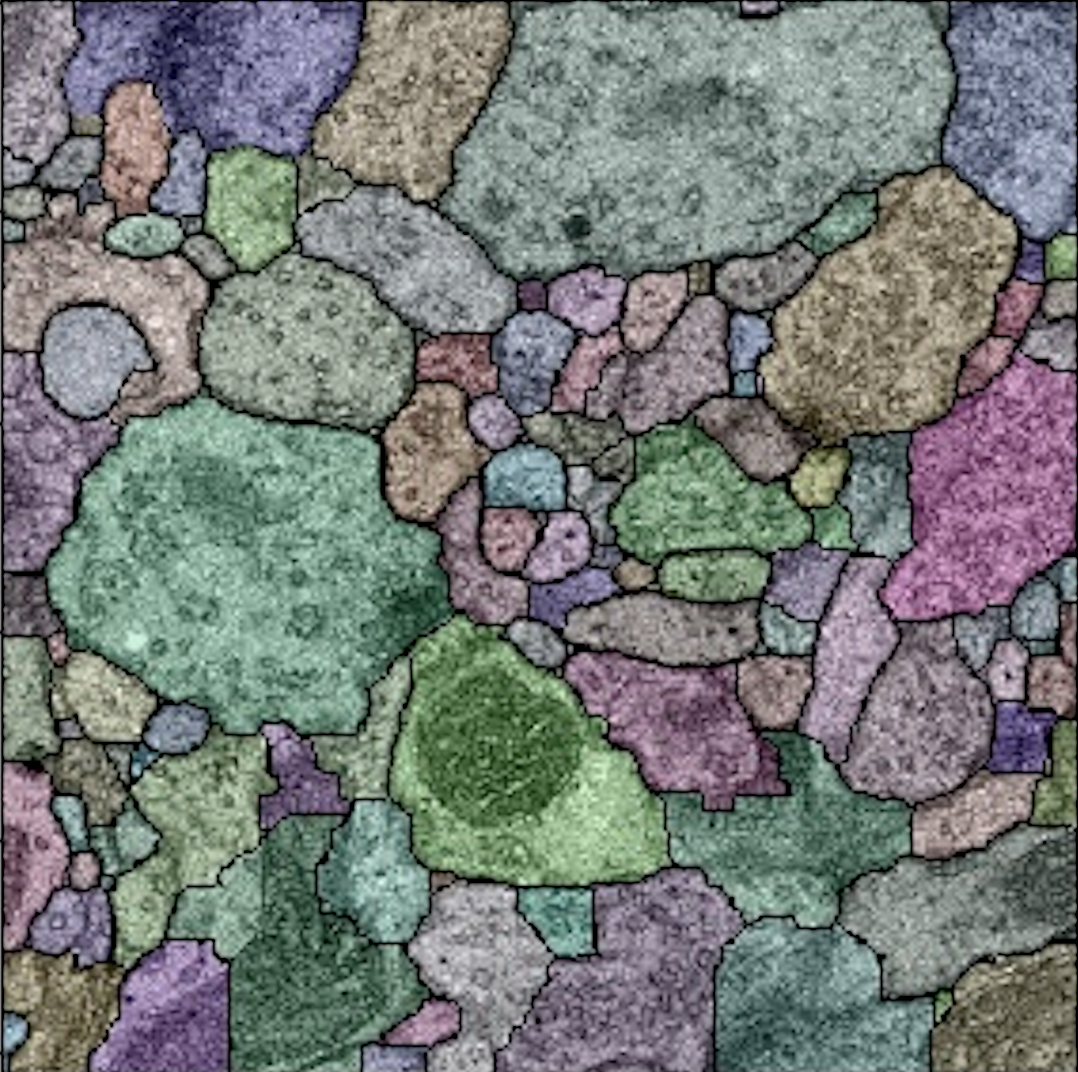
\includegraphics[width=.9\linewidth]{oi2}
  \caption{Original Inference}
  \label{fig:ai1}
\end{subfigure}%
\begin{subfigure}{.3\textwidth}
  \centering
  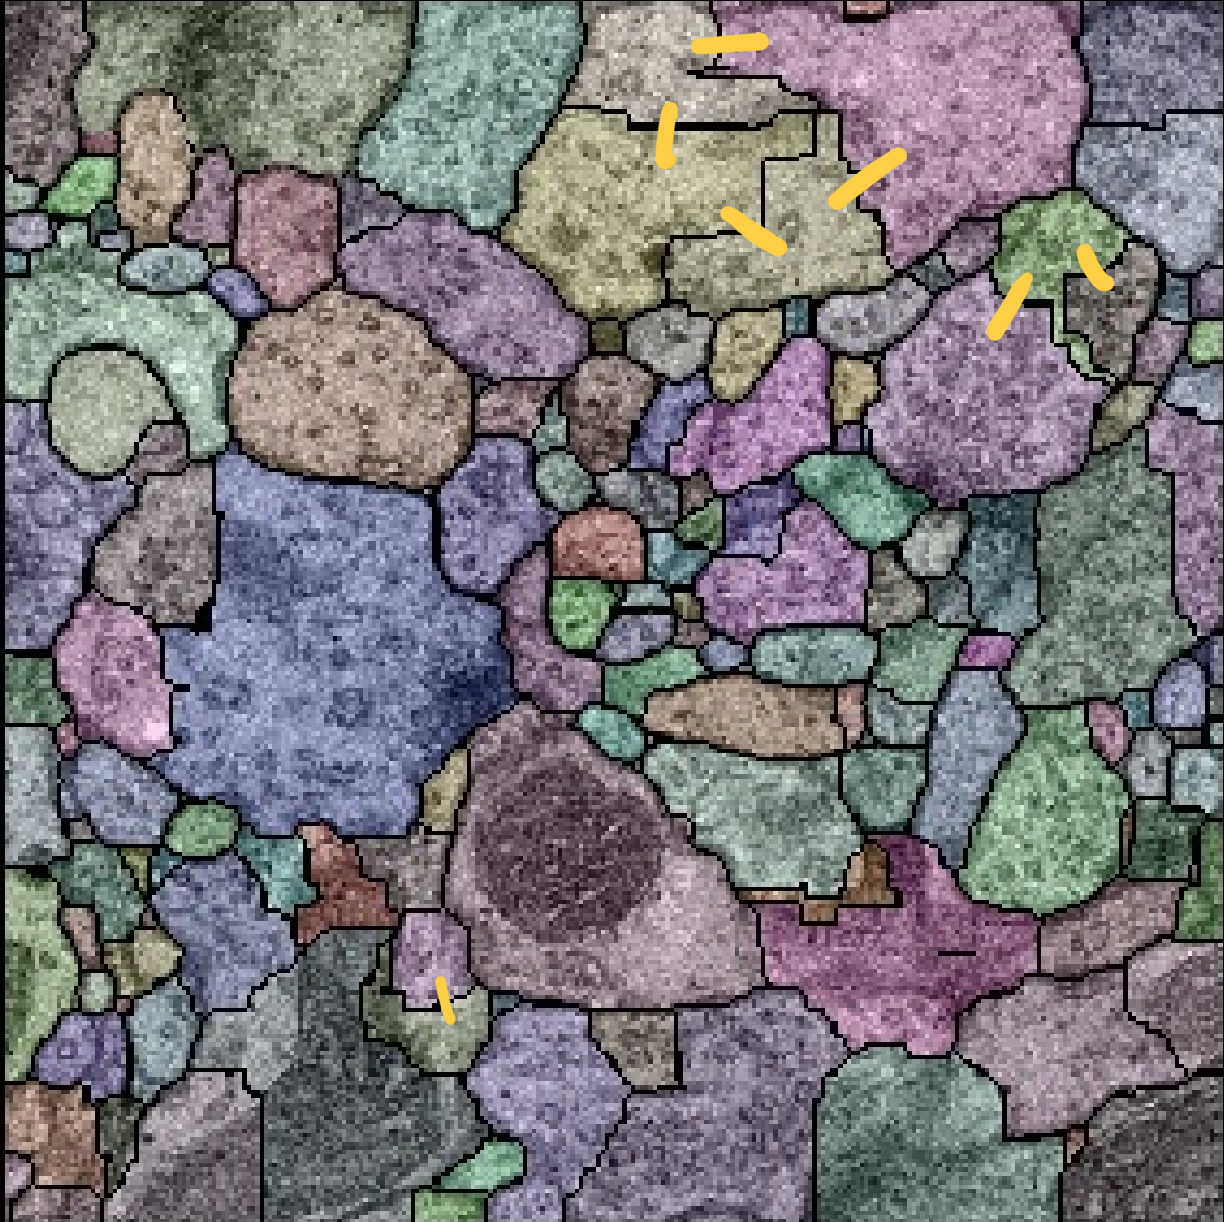
\includegraphics[width=.9\linewidth]{600}
  \caption{Augmented inference}
  \label{fig:ai2}
\end{subfigure}
\begin{subfigure}{.3\textwidth}
  \centering
  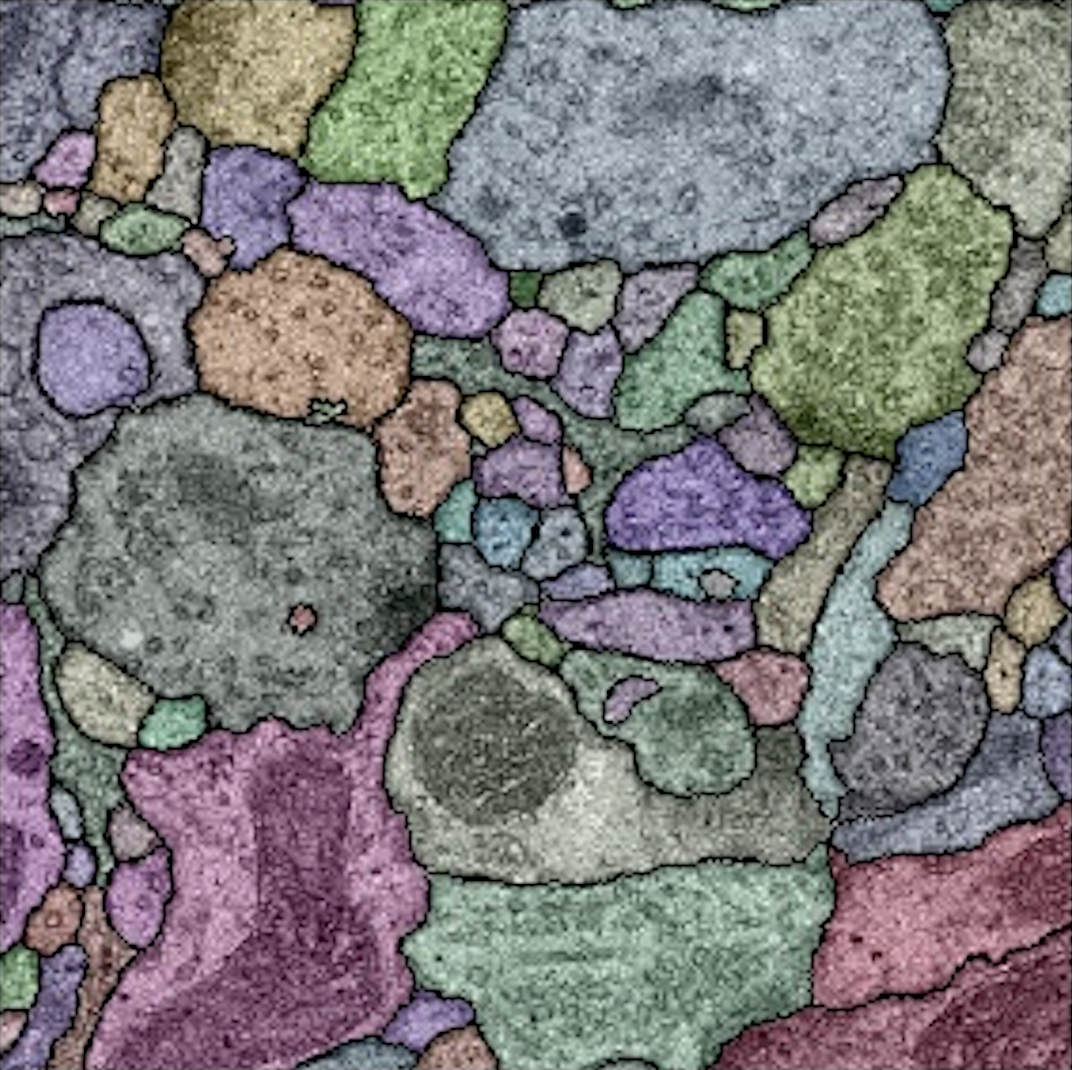
\includegraphics[width=.9\linewidth]{oi3}
  \caption{Ground Truth Image}
  \label{fig:ai3}
\end{subfigure}

\label{fig:augmented_inference}
\caption{Inference result with the augmented dataset}
\end{figure}

As it can be seen in figure \ref{fig:ai2}, not only the inference did not improve in the lower areas of the image comparing to the original inference, but also there are other edges that need to be cut in the upper part of the image(marked with yellow marker on figure \ref{fig:ai2}). %In order to have a better evaluation of the new inference, two testing criteria are being used. The first is 

As it can be seen from the stylized neuron images in Github repository, some of the styles aren't that much good and result in a washed out neuron images, examples of these are brought here with their style image along:

\begin{figure}[h]
\centering
\begin{subfigure}{.3\textwidth}
  \centering
  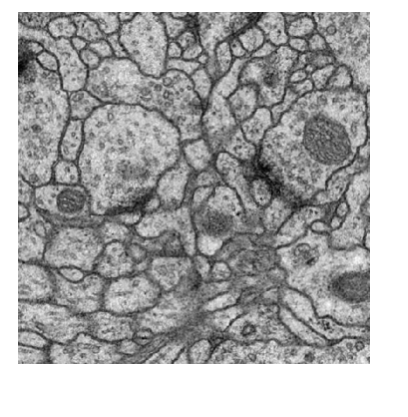
\includegraphics[width=.9\linewidth]{wo1}
  \caption{Raw image}
  \label{fig:wo1}
\end{subfigure}%
\begin{subfigure}{.63\textwidth}
  \centering
  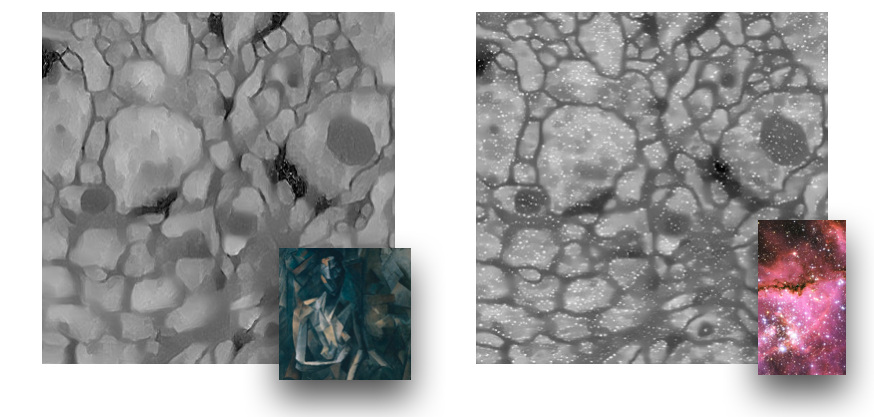
\includegraphics[width=.9\linewidth]{wo2}
  \caption{Stylized images}
  \label{fig:wo2}
\end{subfigure}
\caption{Examples of stylized images that went wrong.}
\label{fig:washedout}
\end{figure}

So this made me think to apply the inference with selected stylized neuron images, and also with a specific stylized image, and combination of original image and a specific stylized image. Results wasn't satisfying in either cases. 

Up until now we showed the result with visualizing it and seeing how the inference was working, however, in order to have a complete evaluation of the results, two testing criteria are being utilized, Random Error and Variation of Information Error which both are implemented in NIFTY software library. The above mentioned test scenario's along with the error measurements are plotted in figure \ref{fig:error}. Unfortunately, as the figure shows, I couldn't get any improvement and using the original dataset has the lowest error comparing to other implemented scenarios. Among the implemented scenarios, using the original dataset plus one  specific stylized image works the best which makes sense because the random forest probably still using the features from the original dataset. As it was expected, using a selected stylized images work better that using all the dataset together. 

\begin{figure}[H]
\centering
\begin{subfigure}{.45\textwidth}
  \centering
  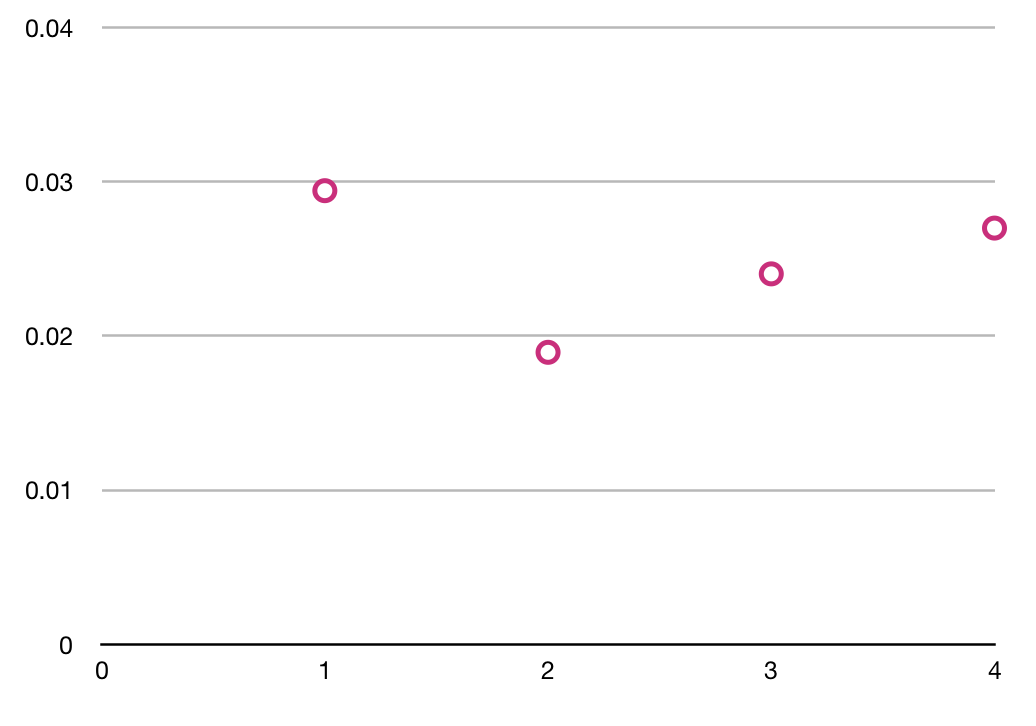
\includegraphics[width=.9\linewidth]{error1}
  \caption{Random Error}
  \label{fig:error1}
\end{subfigure}%
\begin{subfigure}{.45\textwidth}
  \centering
  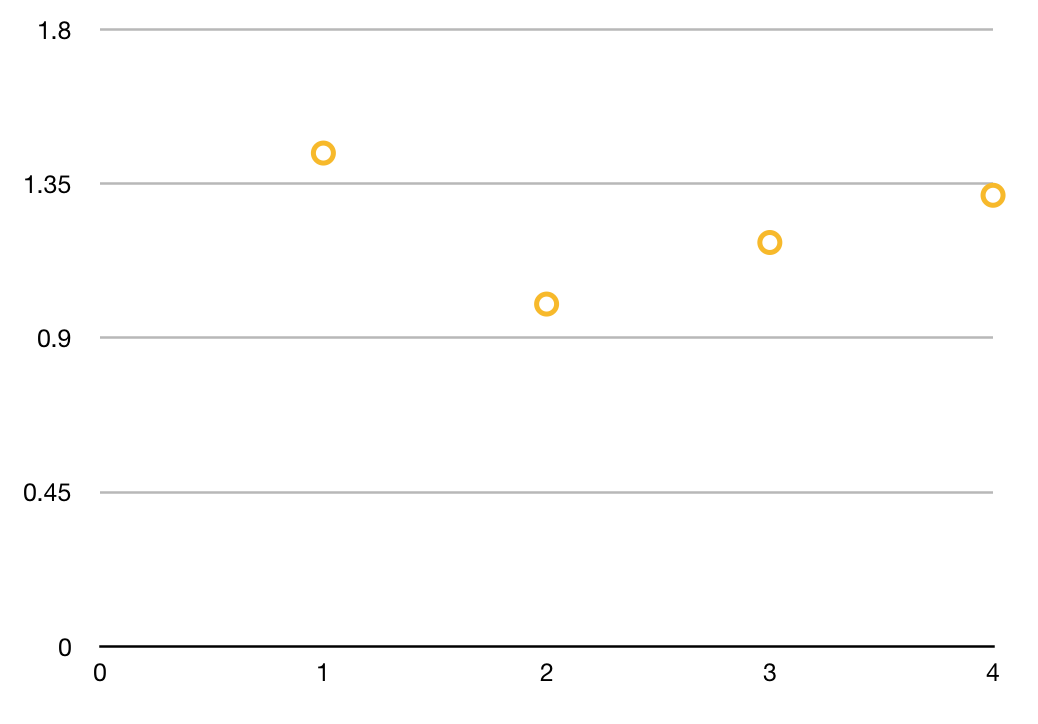
\includegraphics[width=.9\linewidth]{error2}
  \caption{Variation Of Information Error}
  \label{fig:error2}
\end{subfigure}
\caption{Different Scenarios Error Measurements; 1. Full Augmented Dataset, 2. Original Dataset, 3. Original Dataset + Specific Stylized Image, 4. Selected Stylized Images }
\label{fig:error}
\end{figure}

%%%%%%%%%%%%%%%%%%%%%
\section{Summary }

An attempt to improve the inference problem on the ISBI Challenge has been done using Deep Style Transfer. The focus was some how to improve the results by augmenting the dataset with other styles images. Unfortunately no clear improvement  has been obtained. The reason behind this might be mostly because the style transfer does not really introduce \emph{informative} images to the Random Forest Classifier. Moreover, some undetectable changes might occured in specific areas of the data set when the style transfer implemented and this might resulted in miss alignment with the ground truth images.
\label{sec:sum}

\bibliographystyle{ieeetr}
\bibliography{bibliography}

\end{document}
